
\chapter{Etapas propostas no Plano de Trabalho} \label{Etapas}
As etapas do plano de trabalho buscou direcionar as atividades de pesquisa de modo que a cada passo o bolsista conseguisse formar uma base sólida de entendimento da sua área de pesquisa. A fim de alcançar os objetivos do Projeto de Pesquisa as etapas a seguir foram estipuladas:
\begin{enumerate}
    \item  Estudo bibliográfico das perspectivas nacional e internacional no que diz respeito a veículos autônomos;
    \item  Pesquisa bibliográfica para compreender o que busca economicamente e tecnologicamente o mercado internacional e nacional em relação a veículos autônomos;
    \item Aprender quais são os diferentes tipos de veículos autônomos;
    \item Pesquisa bibliográfica das tecnologias essenciais de um carro autônomo;
    \item Mapear e entender os principais softwares de controle de um carro autônomo;
    \item Elaboração do Relatório Final.
\end{enumerate}

No decorrer desse ano de pesquisas foi possível desenvolver, de forma satisfatória, todas as etapas do projeto. Contudo, a etapa 5 devido a sua grandiosidade necessita de uma pesquisa única e mais aprofundada. De modo a aprofundar e consolidar os conhecimentos do bolsista na área de software para a direção autônoma.

\newpage
\chapter{Objetivos} \label{Objetivos}
\section{Objetivo Geral}\label{Objetivo Geral}
Neste primeiro ano, os nossos objetivos foram documentar e entender o cenário de Veículos Autônomos no mundo e nesse processo contrastar com o brasileiro. De modo, a compreender o cenário automobilístico e suas expectativas para essa categoria de veículos. Portanto, foi buscado identificar as principais diferenças entre esses veículos e o que se espera economicamente e tecnologicamente dessa tecnologia, tanto para o Brasil e o mundo. Por fim, mapeamos quais são os principais recursos tecnológicos que fazem esses veículos possíveis. 

\section{Objetivos em Específico}\label{Objetivos Específicos}
\begin{enumerate}
    \item  Entender o cenário de Veículos Autônomos no mundo, e contrastar com o brasileiro:
    \begin{enumerate}
        \item Compreender o cenário automobilístico brasileiro, e as suas expectativas para essa tecnologia.
        \item Contrastar o mercado de veículos autônomos mundial com o brasileiro, buscando  decifrar o que é necessário para a aplicação dessa tecnologia no país.
    \end{enumerate}
    \item  Estudar as principais empresas de pesquisa que trabalham com Veículos Autônomos no mundo, e o que buscam economicamente e tecnologicamente no setor:
    \begin{enumerate}
        \item Identificar se buscam diferentes tipos de Carros Autônomos. Assim como entender as suas possíveis principais diferenças.
        \item Entender o que essas empresas buscam alcançar economicamente, e tecnologicamente ao inserir essa tecnologia no mercado.
        \item Conhecer as mudanças econômicas que carros autônomos podem trazer para a sociedade brasileira. 
    \end{enumerate}
    \item Mapear as tecnologias essenciais para a Direção Autônoma:
    \begin{enumerate}
        \item Documentar quais são os Softwares, algoritmos de controle, e sensores usados nesses veículos.  
    \end{enumerate}
\end{enumerate}

\newpage
\chapter{Metodologia} \label{Metodologia}
Utilizamos uma metodologia, com o fim de revisar a literatura existente, que tem como essência desenvolver e colocar o bolsista em contato direto com todo material já desenvolvido em relação a esta iniciação científica, constituído principalmente de: artigos científicos, cursos online, publicações em periódicos, jornais online, monografias e dissertações.

Nesse formato metodológico, pesquisa bibliográfica, foi possível ter contato e se fundamentar com os principais materiais da atualidade relacionados a veículos autônomos. De modo a ter contato com o que há de mais recente sobre o assunto.

Ressaltamos que, com o decorrer das pesquisas, foram encontradas fontes relevantes, que já possuem mais de 3 anos desde sua publicação. Devido a isso, o bolsista tomou essas publicações como ponto de partida para atualizar-se sobre o que há de mais novo sobre o assunto, de maneira a sempre manter o conteúdo deste relatório o mais atual possível.

A pesquisa bibliográfica seguiu as seguintes etapas \cite{bibli}: 

\begin{figure}[H]
\centering
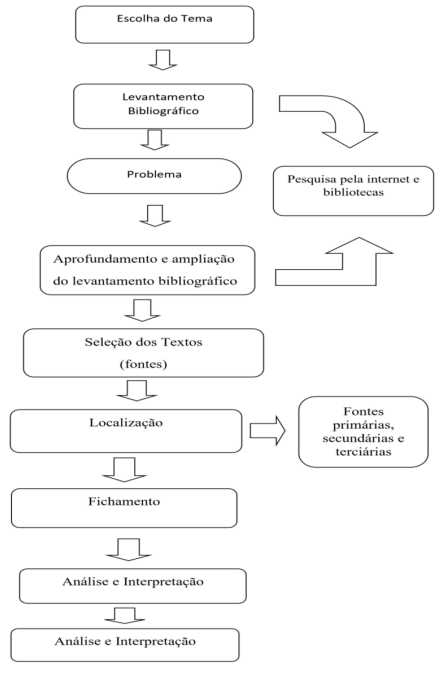
\includegraphics[width=8cm]{Figures/bibli.png}
\caption{Etapas da pesquisa Bibliográfica.}
\label{img_bibli}
\end{figure}

As etapas apresentadas acima foram seguidas pelo bolsista de modo a auxiliá-lo na
delimitação do tema a ser pesquisado e em sua organização.

\vspace {1cm}


A seguir forneceremos detalhamento para as etapas (Figura \ref{img_bibli}) da pesquisa bibliográfica desenvolvida neste projeto:

\vspace {1mm}


\begin{itemize}

\item \textbf{Escolha do tema:} A escolha do tema foi feita no desenvolvimento do Plano de Trabalho para essa Iniciação Científica; Veículos Autônomos e suas tecnologias. 

\item \textbf{Levantamento Bibliográfico:} O bolsista fez o seu levantamento preliminar através dos seguintes meios na internet (Google academic, Google livros, biblioteca virtual, bibliotecas, site das bibliotecas de universidades, CAPES e outros). Foram pesquisadas referências na plataforma scholar.google.com, no portal do Periódico CAPES, e jornais e artigos pela internet. A busca nos bancos de dados abrangeu os anos de 2022 a 2023. Contudo, a partir de pesquisas na internet, também, fizemos uso de materiais publicados a partir de 2019. Como palavra-chave utilizou-se os termos: Autonomous Vehicles, Autonomous, Cars, Mobility, Connected Car, AV, TaxiBot, e self-driving cars.  A pesquisa limitou-se nos idiomas inglês, português,  alemão, e espanhol (ordenado por mais uso).


\item \textbf{O problema:} Devido ao enquadramento dessa pesquisa, por visar unicamente o enriquecimento do bolsista sobre os materiais já desenvolvidos sobre o tema. Este trabalho não busca responder, necessariamente, a um problema de pesquisa. Devido a isso, podemos enquadrar nossos Objetivos (seção \ref{Objetivos}) nessa etapa, de modo a ser nossa estrela guia para desenvolver a pesquisa.

\item \textbf{Aprofundamento e ampliação do levantamento bibliográfico:} Buscamos por obras (artigos, teses, matérias) mais recentes, dos últimos 3 anos, para nos mantermos atualizados evitando conteúdos obsoletos. Mantivemos um número razoável de fontes bibliográficas, de modo que o bolsista não se perdesse durante o desenvolvimento de sua pesquisa. 

\item \textbf{Seleção das fontes:} Houve a seleção das fontes mais relevantes para o projeto a partir de filtros: o primeiro filtro ocorreu pela leitura dos seus títulos, sendo selecionados os que se referiam as palavras-chave apresentadas no \textit{Levantamento Bibliográfico}. A segunda filtragem foi realizada a partir da leitura dos resumos. Neste filtro foi possível identificar publicações que apresentaram relevância para o nosso tema.
Portanto, por meio de uma leitura crítica o bolsista buscou assimilar as obras levantadas, sempre analisando se faria sentido usá-las para o desenvolvimento do projeto. 

\item \textbf{Localização das fontes:} Como apresentado na etapa de  \textit{Levantamento Bibliográfico} estaremos fazendo uso de recursos online para este projeto. Sobretudo, da plataforma CAPES.

\item \textbf{Fichamento:} Para este projeto não foi realizada a classificação dos artigos encontrados. Entretanto, nessa etapa, foram feitos resumos e rascunhos de modo a auxiliar o bolsista no firmamento de seus conhecimentos, e no desenvolvimento do relatório final.

\item \textbf{Análise e Interpretação:} Buscamos averiguar se os materiais encontrados contém valor teórico para o projeto, se sofreu alterações, interpolações, e possíveis falsificações ao longo do tempo. Houve, também, a checagem das fontes dos materiais apresentados, de modo a sempre buscar pela fonte principal do assunto, e nos principais meios de mídias globais.


\end{itemize}

 
Como apresentado no plano de trabalho, a Iniciação Científica buscou seguir um princípio metodológico “Project-based learning” \cite{krajcik2006project}, que visa construir soluções a partir de problemas reais em nossa sociedade. Visto que, é uma modalidade de estudo que deixa as pessoas envolvidas livres para seguir a sua curiosidade, desejo de resolver os problemas encontrados pelo caminho e de buscar por mais informações para resolvê-los, contempla os objetivos desejados para a realização de maneira satisfatória deste projeto. 

Além disso, as pesquisas fundamentam-se no método de pesquisa Revisão Sistemática de Literatura (RSL) que segundo Maria Cristiane \cite{revi3}, e Nakano \cite{revi2} refere-se a um tipo de investigação que se concentra em uma questão bem definida, visando identificar, selecionar, avaliar e sintetizar as evidências disponíveis relacionadas a uma questão formulada de interesse para o pesquisador, esse princípio e método foram utilizados nas etapas definidas na figura \ref{img_bibli} .

Por fim, enaltecemos que devido ao formato de pesquisa, as fontes do bolsista foram crescendo com o passar do tempo e de suas pesquisas. Portanto, o seu levantamento bibliográfico encontra-se muito mais rico comparado com o início de sua seleção bibliográfica.


\vspace {1cm}

O bolsista, também, utilizou dos seguintes formatos de aprendizado durante o desenvolvimento do projeto.
\begin{itemize}
\item \textit{Cursos e minicursos;}
\item \textit{Participação em eventos.}
\end{itemize}

\newpage

\chapter{Resultados e Discussão} \label{resultados}

\section{Veículos Autônomos no Brasil e no mundo}

Nesta seção tratamos do potencial transformativo dos VAs, focamos em pesquisas que nos trouxeram tendências, benefícios, e problemas para implementação de VAs no Brasil e no mundo. No aspecto de implementação, foi possível identificar setores da sociedade em que VAs podem ser amplamente utilizados e áreas em que já são aplicados na atualidade. Ademais, durante as pesquisas, foi encontrado relatórios e artigos que nos trouxeram uma visão analítica do cenário de VAs para 30 países do mundo, nos enriquecendo com dados concretos do cenário atual para essa categoria de veículos. 

\subsection{Implementação de Veículos Autônomos no Brasil e no Mundo}

Antes de entendermos como implementá-lo, precisamos entender quais são esses veículos: Veículos autônomos são todos os veículos que não exigem um motorista humano de maneira parcial ou total para conduzi-los, ou seja, veículos que podem dirigir sozinhos. Alguns veículos que podem ser considerados autônomos já fazem parte do cotidiano de certas cidades, são os metrôs e trens que não precisam de motorista, ou o motorista só está ali para casos extremos. No entanto, com os últimos avanços e inovações tecnológicas, a automação está se expandindo não apenas para trens, mas também para carros, caminhões, ônibus, escavadeiras (entre outros veículos industriais) e até barcos, navios e aviões. Com a automação desses meios de transporte, o mundo experimentará uma reviravolta sem precedentes \cite{4cenarios_ocidental}.

Nesse aspecto, o estudo de sua implementação, a ser desenvolvido nos próximos subcapítulos, é fundamental para compreendermos quais âmbitos da nossa sociedade essa categoria de veículos podem ser alocados, e os benefícios e dificuldades de sua implementação no Brasil e no mundo.

 \subsubsection{Expectativas com a implementação dos Veículos Autônomos}
Devido ao seu potencial transformativo, vários benefícios são esperados. Entre esses benefícios e expectativas estão o de redução de acidentes de trânsito. Estima-se que no brasil o número de mortes em acidentes de transporte terrestre no período de 2019 foi de 31.945 \cite{Anexo_I_pnatrans}. Veículos autônomos vêm com a promessa de buscar uma redução nesses números através da retirada do principal causador de acidentes de trânsito: erros humanos. 

Ademais, Veículos Autônomos vem como uma forma de minimizar os congestionamentos nas grandes metrópoles. Segundo o  Plano Estratégico de Desenvolvimento Urbano Integrado da Região Metropolitana do Rio de Janeiro, \cite{rj_transito}, apenas na hora do rush da manhã o fluxo de viagens de São Gonçalo a Niterói chega a quase 100 mil pessoas sendo transportadas; desses deslocamentos cerca de 80\% das viagens são feitas em transporte público – ônibus convencionais. Diante disso, uma das propostas para suprir essa demanda de transporte seria a inclusão de veículos autônomos. Nesse formato, carros poderiam ser solicitados como, hoje, são feitas as corridas de aplicativos, e os ônibus do transporte público  poderiam operar por mais horas e com menor custo. 
Entretanto, ainda seria necessário lidar com outros problemas como a disputa de espaço nas vias, e os engarrafamentos crônicos das cidades; De acordo com informações do levantamento domiciliar realizado durante a elaboração do último PDTU, o tempo médio de deslocamento do centro de São Gonçalo a Niterói é de 50 minutos, devido a problemas relacionados ao grande fluxo de veículos, sendo o transporte público quase 25\% maior. Diante disso, os veículos autônomos teriam que disputar espaço nas vias com veículos ainda conduzidos por pessoas. Sabendo que essa categoria será e está sendo implementada de maneira gradual na sociedade, começando por veículos de luxo \cite{caio}.

\begin{figure}[H]
\centering
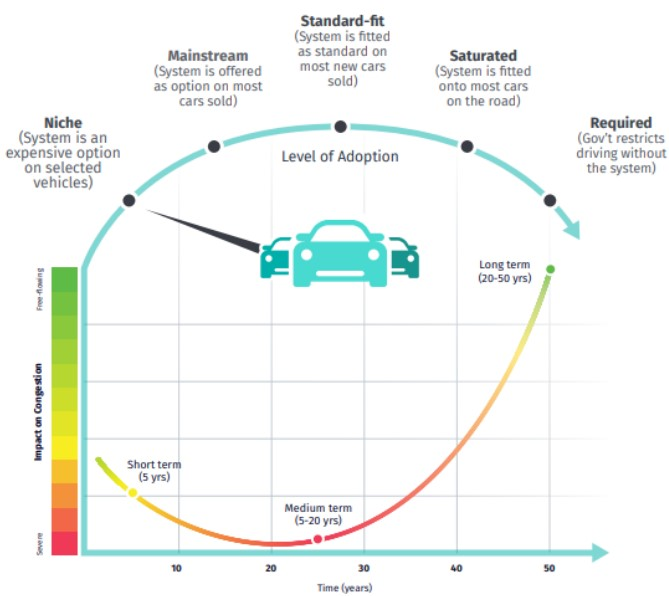
\includegraphics[width=10cm]{Figures/conge.jpg}
\caption{Impacto dos níveis de autonomia no congestionamento ao longo do tempo \cite{4cenarios_ocidental}.}
\label{congestionamento}
\end{figure}

Um estudo de casos considerado um cenário onde veículos autônomos têm que lidar com congestionamentos, levaram à conclusão de que o aumento do número de veículos autônomos, totalmente conectados, dirigindo em pelotões dentro de uma rede, reduz os atrasos e congestionamentos. Como resultado, mantém ou melhora o tráfego da rota escolhida no estudo. O veículo líder do pelotão foi capaz de antecipar mudanças nos sinais e comunicá-los com os veículos de trás, permitindo-lhes um melhor desempenho em cruzamentos sinalizados. Os pelotões também aumentaram a capacidade de rede em links congestionados, permitindo melhor desempenho nos atrasos médios \cite{conge}.

Mapa da visão geral dos benefícios, riscos e mudanças incertas com a aplicação dos VAs na sociedade:

\begin{figure}[H]
\centering
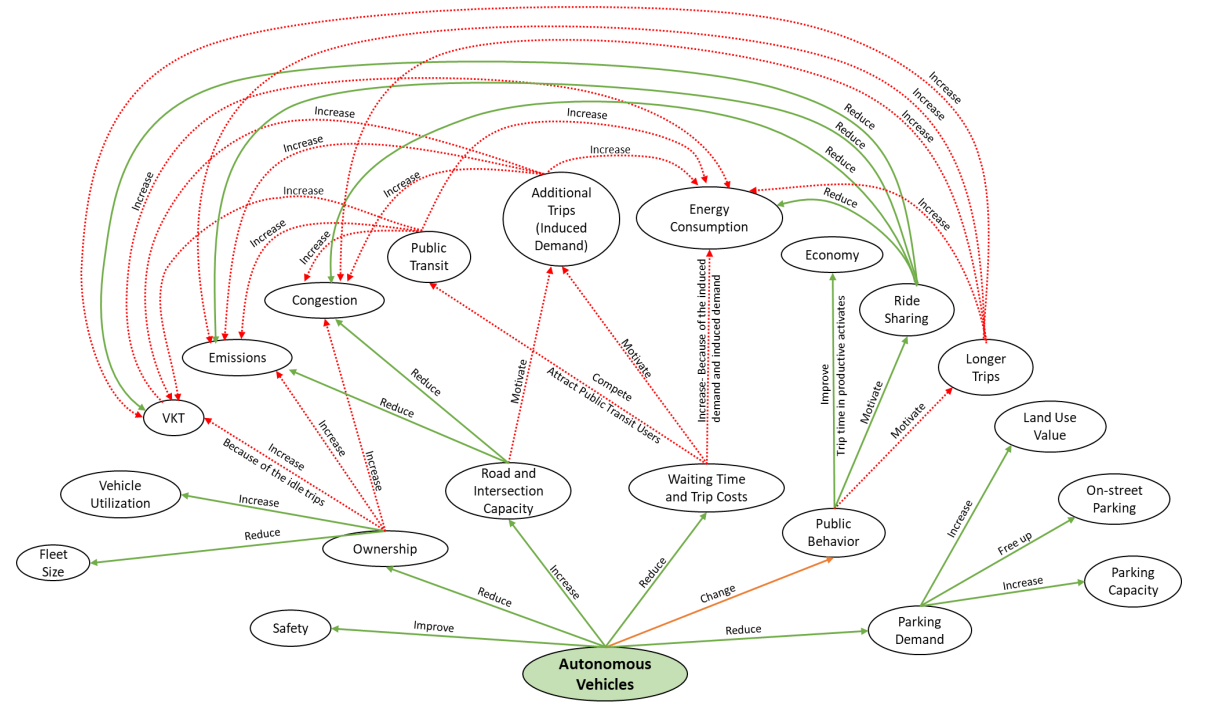
\includegraphics[width=16cm]{Figures/map.png}
\caption{Mapeando a relação entrelaçada entre as implicações dos VAs (verde = benefício, vermelho = risco, laranja = mudança incerta) \cite{mundobrasil}.}
\label{mapa_resumo}
\end{figure}


\subsubsubsection{Implementação em setores industriais}

Ainda tratando sobre benefícios em veículos
autônomos em nossa sociedade.
Há a utilidade dessa categoria em ambiente industrial, onde poderiam  operar em indústrias automotiva, indústria de bebidas, indústria eletroeletrônicas, implementos agrícolas, porto, linha de montagem, almoxarifado, etc.

A aplicação de veículos autônomos em portos é uma solução que visa aumentar a eficiência do transporte de contêineres e materiais para os navios e setores de portos. O uso desses veículos aumenta a automação de movimentação logística, acelerando o processo de carga, descarga e armazenamento de carga. Fazendo com que a produção tenha um ganho significativo 
na competitividade do mercado, aumento da produtividade e redução de custos das indústrias, na qual esforçar-se para otimizar os processos de manuseio de materiais por meio da automação, essas máquinas podem atuar de maneira ótima em rotas programadas tanto na função de abastecimento nas linhas de produção quanto na transferência entre estações ou áreas do processo produtivo e no transporte de matéria-prima ou produto acabado \cite{aplicacao}.

\subsubsection{Veículo Autônomo e áreas de implementação} \label{implementacao}

Devido a sua simplicidade, segurança e conforto em operação. Podem ser aplicados em diversas áreas e setores da sociedade, como na execução de funções e tarefas de risco e que  seres humanos não seriam capazes de realizar, ou na execução de funções exaustivas, onde o ser humano teria uma menor eficiência. Visto que a maioria desses veículos  tem suas funções executadas automaticamente, necessitando de nenhum ou pouca supervisão de um humano. 
Os tornando perfeitos, também, para pessoas com deficiência e idosos viverem suas vidas de forma mais independente. 
\vspace {1cm}

Aplicações especializadas de veículos autônomos \cite{aplicacao2}:

\begin{enumerate}
 \item \textbf{Transporte público:} O Veículo Autônomo (VA) foi introduzido inicialmente no sistema de transporte público na modalidade de operação sem condutor. Hoje em dia, as tendências modernas no transporte público são úteis na região metropolitana para os turistas, próprios cidadãos, etc. Como visto, o transporte é um grande desafio em áreas lotadas, apertadas e desordenadas em várias cidades. Ainda assim, devido à introdução de veículos elétricos autônomos, é possível gerenciar os problemas em locais congestionados. Como mencionado anteriormente, um dos benefícios do trânsito sem motorista seria o melhor serviço para passageiros com deficiência. O serviço de transporte para pessoas com deficiência geralmente é inconveniente, não confiável e caro. Os passageiros com deficiência geralmente precisam reservar uma viagem 24 horas antes da partida e são informados de que a coleta pode ocorrer a qualquer momento durante uma janela de 2 horas \cite{notif}.
\item \textbf{Bonde e Trem Elétrico Autônomo:} O primeiro veículo sobre trilhos elétrico automatizado foi projetado e desenvolvido pela Siemens na Alemanha. Em 2018, o primeiro test drive do bonde foi realizado na Alemanha por sete quilômetros. O uso de dispositivos inteligentes, como câmeras inteligentes, sensores inteligentes e sistemas LiDAR inteligentes baseados em software, é útil para o bonde dirigir em áreas lotadas de várias cidades sem nenhum obstáculo. Devido ao algoritmo inteligente, sistemas inteligentes de monitoramento e controle, um bonde operará com segurança mesmo em áreas lotadas. Diante de qualquer obstáculo, o bonde se encarregará de solucionar a situação com o auxílio de outros aparelhos auxiliares, iniciando-se o trajeto imediatamente após a retirada do obstáculo do seu caminho. Nesse mesmo sentido, houve o Harry projetado e desenvolvido em 2017, na Inglaterra.Visando suprir a falta de transporte público em algumas localidades de Londres.
\item \textbf{Helicóptero Elétrico Autônomo:} O VSR700 é um dos protótipos inovadores de Helicópteros Elétricos Autônomos inventados em 2020 pela Airbus em um teste pesado na França. Ele é projetado e desenvolvido para operar ao lado de vários meios navais. O objetivo é fortalecer os navios, aumentar seu escopo usando sensores inteligentes em associação com helicópteros e aprimorar o cenário de coleta de informações das perspectivas do navio. Os Helicópteros Autônomos estão fazendo o trabalho de vigilância das informações de seus alvos e confirmando o destino de chegar aos navios nos locais desejados. 
\item \textbf{Caminhão Inteligente Autônomo:} Um caminhão elétrico totalmente automatizado foi projetado e desenvolvido em 2016 com o nome Otto. Sem motorista humano, opera com a ajuda do sistema LIDAR. Esses caminhões modernos minimizam os acidentes e são utilizados para entrega de mercadorias e serviços pesados. Além disso, o caminhão elétrico autônomo Vera, um Volvo, foi projetado e desenvolvido para transportar mercadorias de diversos destinos, como indústrias, estaleiros, minas, portos, pátios de armazenamento e armazéns e possui formas muito eficientes, seguras, limpas e sustentáveis do que os caminhões atuais mais comuns.

\item \textbf{Veículo Subaquático Autônomo:} É usado em estudos geográficos da marinha e também é popular no setor técnico e de defesa. A principal função deste veículo é obter uma imagem aprimorada do fundo do mar com uma resolução muito alta da superfície de uma embarcação, ou objeto de investigação.
\item \textbf{Veículos Autônomos para Agricultura e Mineração:}  Os veículos autônomos são usados no setor agrícola para vários processos agrícolas e usados em tarefas operacionais de mineração. Diferentes tipos de veículos autônomos de agricultura e mineração são tratores agrícolas autônomos, veículos terrestres não tripulados usados para fazendas inteligentes, veículos de mineração, como caminhões de mineração, máquinas automatizadas de mineração, etc.

\end{enumerate}

Ainda na perspectiva de implementação, os VAs podem ser introduzidos no âmbito de veículos de entrega, transporte público, e em um contexto de pandemia na detecção de infectados.

\begin{figure}[H]
\centering
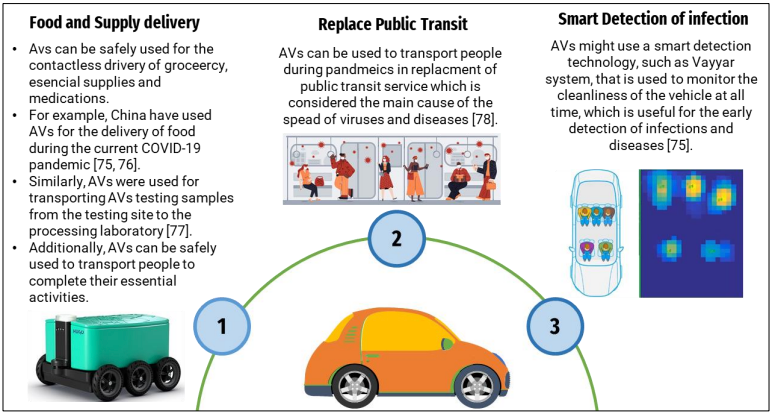
\includegraphics[width=\textwidth]{Figures/aplic.png}
\caption{Resumo dos benefícios dos VAs e aplicações \cite{mundobrasil}.}
\label{resumo_aplic}
\end{figure}

\begin{quote}

Descrição da figura (Figura \ref{resumo_aplic}) apresenta um resumo de 3 aplicações com os VAs, sendo essas:

\begin{enumerate}
 \item \textbf{Entrega de suplementos e comidas:} Apresentando que os VAs podem ser uma alternativa segura e útil para a entrega de medicamentos, suplementos essenciais, produtos de supermercado. Como exemplo prático, introduz o uso dessas VAs na China durante a pandemia de COVID-19 no transporte de suplementos no geral. Assim como, o uso em laboratório no transporte de material em teste, e no transporte de pessoas.

\item \textbf{Transporte público:} Como visto anteriormente, os VAs são uma excelente alternativa para o transporte da população. 

\item \textbf{Detecção de infectados:} Os VAs podem ser equipados de tecnologias capazes de detectar e monitorar pessoas infectadas no veículo, ou identificar se o VA está sujo e precisando de alguma manutenção. 

\end{enumerate}

\end{quote}

\subsection{O cenário de aplicação de Veículos Autônomos}
Segundo o relatório “2020 Autonomous Vehicles Readiness Index” da KPMG; empresa que opera em 143 países e territórios em todo o mundo, oferecendo serviços de auditoria, impostos e consultoria. Este relatório buscou avaliar a preparação de 30 países e jurisdições na corrida por veículos autônomos, sendo uma ferramenta para ajudar a medir o nível de preparação para veículos autônomos. É um índice composto que combina 28 medidas individuais de uma variedade de fontes em uma única pontuação. Mais informações sobre os resultados, metodologia e fontes utilizadas podem ser encontradas em, \cite{KPMG}.

\begin{figure}[H]
\centering
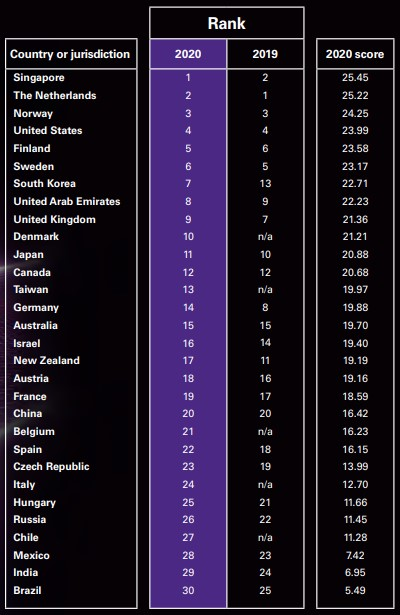
\includegraphics[width=8cm]{Figures/rank.jpg}
\caption{Resultado do relatório 2020 Autonomous Vehicles Readiness Index \cite{KPMG}.}
\label{KPMG}
\end{figure}

Observando o ranking notamos que o Brasil, entre os países estudados, encontra-se na trigésima posição, ficando na última colocação. Dentre os pilares citados e estudados pela KPMG o Brasil apenas não ficou em último lugar na questão de aceitação do consumidor, ficando na vigésima nona posição.
Entre os pontos apresentados o estudo ressalta que o governo brasileira está fazendo muito pouco para encorajar a adoção dos VA, refletindo na última posição do ranking AVRI. Isso apesar do entusiasmo do país por novas tecnologias e serviços, como carona, diz Maurício Endo, chefe de governo da KPMG no Brasil e na América do Sul. “Ainda não vemos nenhuma política pública para criar um caminho para que os VAs comecem a operar nas cidades”.

O programa Rota 2030, lançado em 2018, oferece incentivos para substituir os tipos de motores tradicionais por híbridos ou Veículos Elétricos, embora esse não seja o objetivo principal. Em Outubro de 2019 houve o lançamento de uma pequena frota de carros elétricos Renault Twizy junto com pontos de recarga em Brasília, permitindo que funcionários públicos se desloquem entre prédios do governo de maneira mais econômica e com menos emissões de carbono do que antes.

Por outro lado, o setor privado é mais ativo, embora se concentre nos usos das vias públicas. Em janeiro de 2020, a montadora brasileira de veículos Hitech Electric lançou o que chamou de primeiro VA desenvolvido no país. O e.coTech4 elétrico de dois lugares, que pode atingir velocidades de 50 km/h, está inicialmente disponível apenas para aluguel corporativo em áreas fechadas, como áreas industriais, campus universitários e resorts \cite{KPMG}.

\begin{figure}[H]
\centering
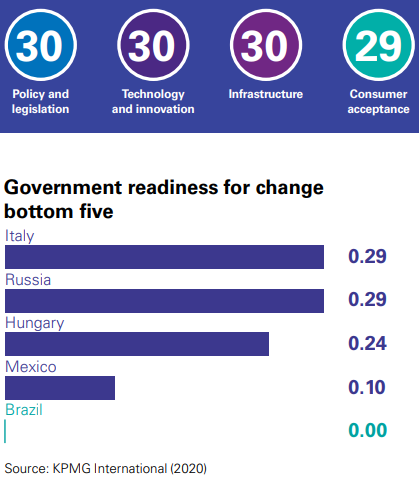
\includegraphics[width=8cm]{Figures/rank30.png}
\caption{Posição do Brasil no relatório \cite{KPMG}.}
\label{rank30}
\end{figure}

Ademais, temos o estudo anual da indústria do \textit{Connected Car Innovation} (CCI) formulou um índex que busca pesquisar empiricamente e comparar o desempenho e a força inovadora de 28 fabricantes globais de automóveis nas áreas de veículos e serviços conectados, bem como sua força de mercado usando vários indicadores. O estudo é baseado no banco de dados de inovação do Centro de Gestão Automotiva (CAM) \cite{CCI}. A partir deste estudo, podemos identificar que o Brasil não encontra-se como uma força inovadora nas áreas de arquitetura veicular, conectividade/infoentretenimento e direção autônoma dos players mais importantes do universo dos carros conectados.


\begin{figure}[H]
\centering
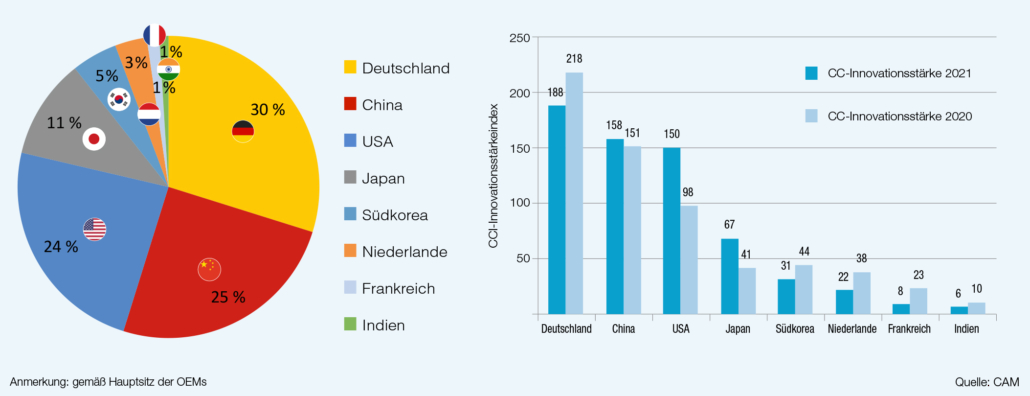
\includegraphics[width=12cm]{Figures/CCI.jpg}
\caption{Força inovadora por país  \cite{CCI}.}
\label{forcaCCI}
\end{figure}


Apesar do pouco encorajamento do governo brasileiro quanto a adoração de veículos autônomos, e a baixa aceitação do Brasil comparado com os demais países da lista. Ainda precisamos tratar sobre questões relacionadas à infraestrutura do país para a navegação e operação desses veículos. 
O principal problema que os VAs enfrentarão são os sistemas de sinalização e marcação precários, gerenciamento de tráfego em caso de incidência de tráfego, gerenciamento de estacionamento, proteção de áreas seguras e heterogeneidade do tráfego.

As figuras abaixo mostram uma discussão detalhada dessas principais barreiras e suas implicações no comportamento dos VAs.
\begin{figure}[H]
\centering
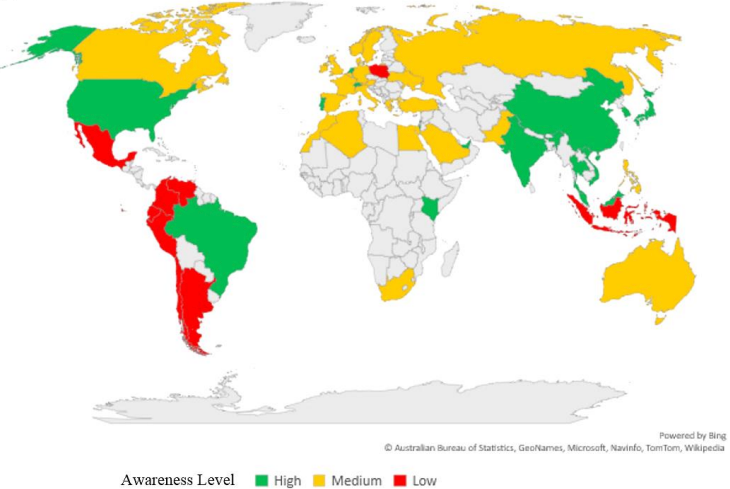
\includegraphics[width=12cm]{Figures/grafik-a.png}
\caption{ Resumo do nível de consciência em diferentes países com diferentes níveis de PIB \cite{mundobrasil}.}
\label{awareness}
\end{figure}
\begin{figure}[H]
\centering
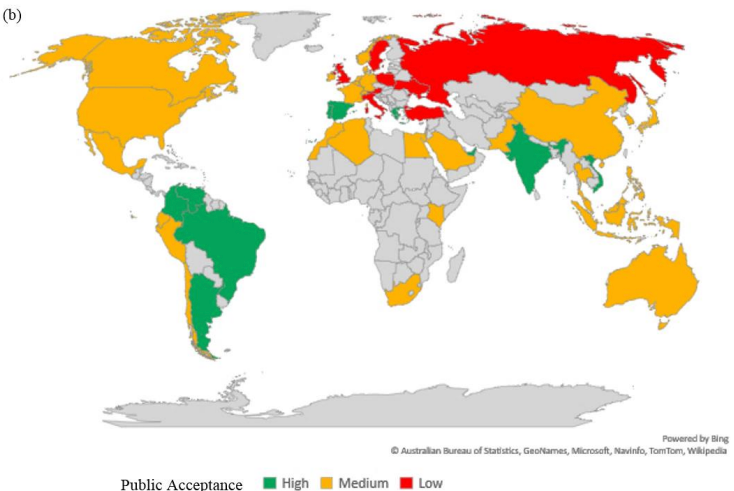
\includegraphics[width=12cm]{Figures/grafik-b.png}
\caption{ Resumo do nível de aceitação pública em relação aos VAs em diferentes países com diferentes níveis de PIB \cite{mundobrasil}.}
\label{public}
\end{figure}

É possível identificar nas figuras \ref{awareness}, \ref{public} que o Brasil encontra-se com um nível alto em consciência e aceitação do público. Para mais detalhes da análise dos principais desafios para a navegação segura de VAs em países em desenvolvimento, \cite{mundobrasil}.

Ainda mais, em outros artigos também podemos identificar que o Brasil tem melhores pontos no quesito infraestrutura comparada com os outros pontos analisados, e ainda se encontra muito atrás comparado com os outros países analisados.
\begin{figure}[H]
\centering
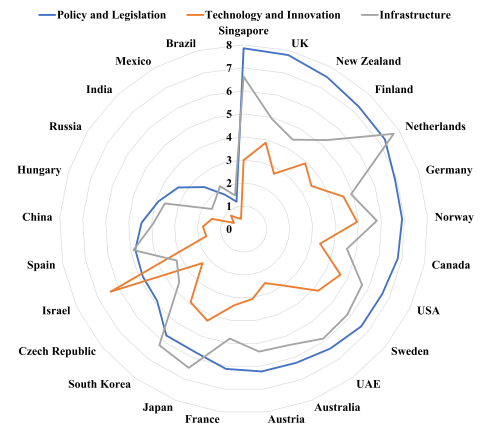
\includegraphics[width=8cm]{Figures/future.png}
\caption{Os sucessos alcançados pelos vinte e cinco principais países até agora em relação aos VAs em termos de política e legislação, tecnologia e inovação e infraestrutura \cite{future-view}.}
\label{figura_future-view}
\end{figure}



Por fim, como identificado nos gráficos \ref{rank30} e \ref{figura_future-view} Singapura foi o país com maior aproveitamento somando os pilares estudados pelo Autonomous Vehicles Readiness Index 2020, tendo em vista os esforços adicionais que tem feito para encorajar o uso de VAs. Em janeiro de 2019, o governo da cidade-estado publicou seu rascunho de padrões nacionais TR68 para esses veículos, bem como uma estrutura voluntária de governança de IA \cite{KPMG}. A KPMG relata que desde o primeiro relatório publicado os países têm apresentado rápidas e fortes mudanças a caminho da implementação e da ampliação das frotas de veículos autônomos, no desenvolvimento de regularizações e incentivos, além de que a mídia começou a considerar as vantagens e desvantagens dos VAs, empresas testam cada vez mais veículos e os consumidores estão aceitando a ideia de migração para Veículos Autônomos.

\section{Veículos Autônomos e suas perspectivas}

Nesta seção tratamos sobre as perspectivas dos VAs em nossas sociedades, identificamos quais são os diferentes tipos de VAs e apresentamos a sua taxonomia com base em fontes reconhecidas mundialmente. Buscamos fazer essa apresentação de maneira bem didática e de forma ilustrativa para uma melhor compreensão de todos. Ademais, trouxemos um panorama de como se encontra o mercado tecnológico e econômico para os VAs; quais são as principais empresas que trabalham e pesquisam nessa categoria de veículos, e quais são as expectativas de lucro de algumas dessas empresas.

\subsection{Nível de condução autônoma}
	
Na busca de identificar os diferentes tipos de Carro Autônomos, nos deparamos com um cenário ainda em processo de definição. Pois, com os presentes avanços na área de veículos autônomos, surgiu a necessidade, das empresas e dos órgãos de regularização, de classificá-los de alguma forma. Desse modo, A SAE (Society of Automotive Engineers), uma das principais associações globais que busca essa classificação, dividiu os veículos autônomos em seis níveis de funcionalidade, que vão desde nenhum recurso de automação (nível 0) até automação completa, sem a necessidade de um condutor humano, (nível 5). Fazendo uso da terminologia “sistemas de direção autônoma” para se referir a veículos que possuem algum tipo de direção autônoma \cite{SAE}. Nesse cenário, os níveis 1 e 2 incluem alguns recursos, enquanto o nível 3 alcança automação limitada, onde o motorista pode abrir mão do controle do veículo, desde que esteja disponível para intervir.

Abaixo, apresentamos graficamente as diferenças de veículos autônomos e suas respectivas classificações \cite{SAE}:

\begin{figure}[H]
\centering
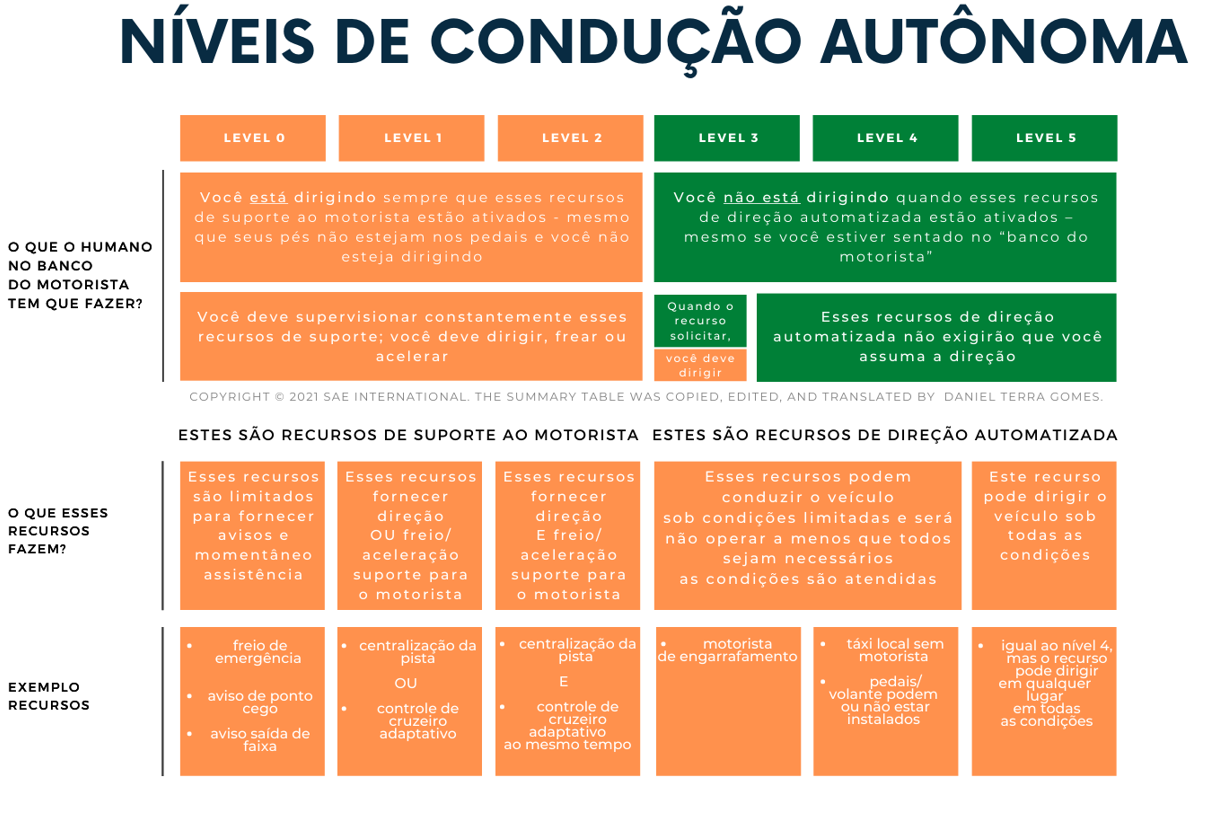
\includegraphics[width=15cm]{Figures/IC-Graph1.png}
\caption{Níveis de Automação de condução PT-BR}
\label{Graph_PT}
\end{figure}
\begin{figure}[H]
\centering
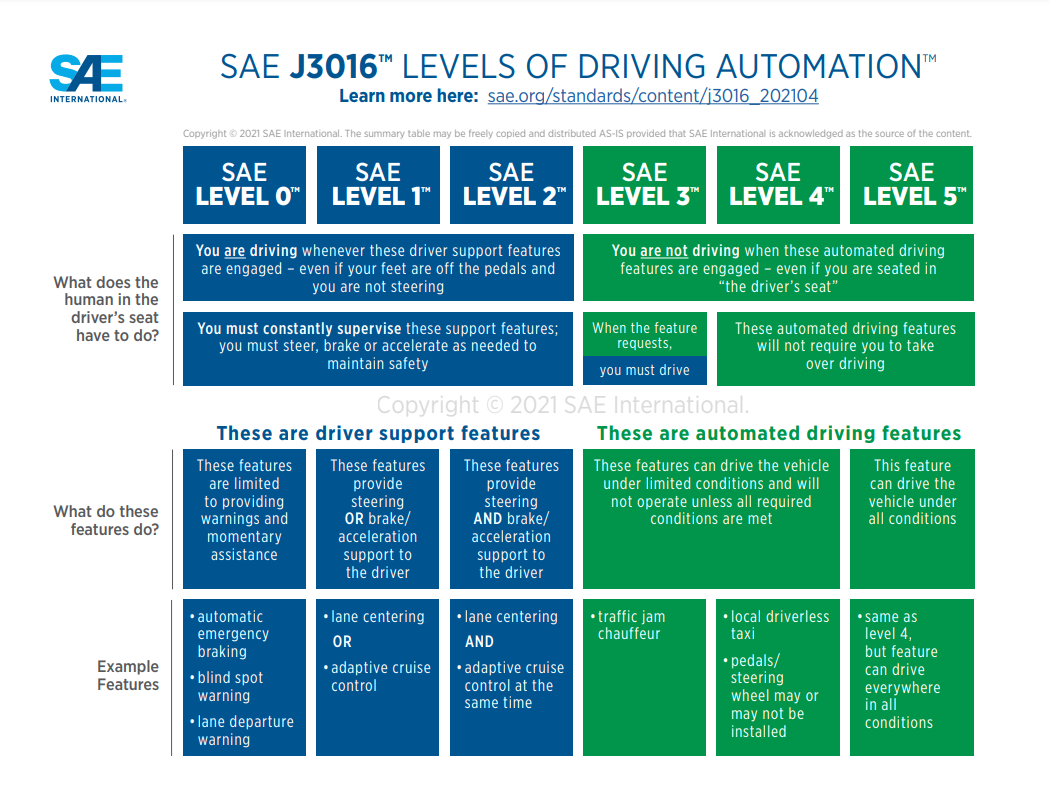
\includegraphics[width=15cm]{Figures/IC-GrapEN.png}
\caption{SAE J3016TM levels of driving automation \cite{SAE}}
\label{Graph_EN}
\end{figure}

Além dessas classificações entre tipos veículos, ainda é possível classificá-los nas seguintes categorias de tipos de automação: Sistema de Assistência Avançada ao Motorista (ADAS) sigla do inglês \textit{advanced driver-assistance system (ADAS)}, ou Condução Automática, Mobilidade Como Serviço (MaaS) sigla do inglês \textit{Mobility as a service (MaaS)}.
Como visto nos gráficos (Gráficos \ref{Graph_PT} e \ref{Graph_EN}) nos níveis 1, 2 e 3 o condutor precisa estar preparado para caso o sistema precise de algum tipo de ajuda do condutor, esses níveis são vistos como uma espécie de remendo pois funcionam como um remendo para suprir uma demanda que os sistemas autônomos ainda não podem cumprir com maestria \cite{4cenarios_ocidental}. Pois com o avanço da tecnologia o condutor humano torna-se cada vez menos necessário, e como visto no nível 5 (Gráfico \ref{Graph_EN}) é possível a retirada do volante do veículo. 

Na atualidade, empresas líderes do setor de veículos autônomos, como a Tesla, ainda trabalham com nível 2 de direção autônoma referente ao ADAS para veículos vendidos para a população. \cite{4cenarios_ocidental}.
Por outro lado, no início deste ano de 2023, a Mercedes-Benz no seu portal de mídias afirma ser a primeira empresa a alcançar a marca de direção autônoma SAE level 3 para o mercado dos Estados Unidos, sendo o estado de Nevada o primeiro a concordar com as regulamentações para a navegação desses tipos de veículos em seu território. A Mercedes afirma, também, que já em 2024 terá os seus primeiros veículos \textit{DRIVE PILOT}, em portugues “condutor”, disponíveis para o mercado Norte Americano.

\begin{quote}
“No mundo moderno, o tempo é um dos bens mais preciosos, e devolver o tempo aos nossos clientes é um elemento central em nossa estratégia de construir os carros mais desejados do mundo. O nosso DRIVE PILOT dá um grande passo para o conseguir e coloca-nos na vanguarda da inovação no campo crucialmente importante da condução autónoma. O DRIVE PILOT demonstra mais uma vez que nosso pioneirismo faz parte do nosso DNA. A certificação em Nevada marca o início de seu lançamento internacional e, com ela, o início de uma nova era.”
Diz o Markus Schäfer, Membro do Conselho de Administração do Mercedes‑Benz Group AG, Diretor de Tecnologia, responsável por Desenvolvimento e Compras \cite{mercedes3}.
\end{quote}

Adicionalmente, algumas empresas, como Waymo e Cruise, atualmente operam serviços de carona com veículos com autonomia de nível 4 nos EUA - isso significa que os carros podem operar sem motorista ao volante sob certas condições, como dentro de uma área de serviço designada, portanto, já mapeadas e entendida pelo algoritmo de controle dos veículos\footnote{Mercedes-Benz wins race to bring Level 3 autonomous cars to US: \url{https://www.freethink.com/hard-tech/drive-pilot}.}.



A seguir forneceremos as definições detalhadas para seis níveis de automação de veículos, variando de nenhuma automação de direção (Nível 0) a automação total de direção (Nível 5), no contexto de veículos a motor, definidos pela SAE \cite{SAE}:

\begin{enumerate} \label{SAE-level}
 \item \textbf{Nível 0} – Sem automação de condução: Não existe nenhum tipo de auxílio ao motorista e nenhuma presença/atuação de tecnologia de condução autônoma, ou assistência.

\item \textbf{Nível 1} - Assistência ao Motorista: No nível 1, o motorista é assistido apenas em relação à velocidade do veículo, um exemplo prático seria o piloto automático, que mantém a velocidade do veículo constante de acordo com o gosto do motorista. Neste caso, o condutor deve continuar a frear, acelerar e direcionar o veículo. Um segundo exemplo seria: o recurso de assistência ao estacionamento, executa automaticamente as ações de controle de movimento do veículo necessárias para estacionar um veículo, enquanto o motorista executa as ações de controle de movimento do veículo longitudinal e supervisiona o recurso de estacionamento.

\item \textbf{Nível 2} - Automação de Condução parcial: Nesta fase, o veículo já é capaz de realizar ações de forma autônoma, como frear, acelerar e parar o veículo em uma direção, como é o caso da tecnologia chamada ACC (Adaptive Cruise Control). No nível 2, o condutor continua a ser responsável pela condução e exige que o condutor esteja atento à condução e retome a condução em situações de perigo. Um exemplo prático seria, como visto: o recurso de assistência ao estacionamento, mas dessa vez, executa automaticamente as ações de controle de movimento lateral e longitudinal do veículo, necessárias para estacionar um veículo sob a supervisão do motorista.

\item \textbf{Nível 3} - Automação Condicional de Condução: Consiste em veículos que são capazes de se mover de forma independente, tanto na direção, aceleração e frenagem. Neste nível de condução, o condutor pode realizar outras atividades enquanto o carro segue autonomamente a sua rota, mas por vezes é acionado para assumir a condução por um curto período de tempo ou para assumir o controlo total em situações de risco. Nesse cenário, um \textit{automated driving system} (ADS)  é capaz de continuar a executar o \textit{dynamic driving task} (DDT) por pelo menos vários segundos após fornecer ao usuário pronto para \textit{fallback}; uma solicitação para intervir. Espera-se então que o usuário pronto para o \textit{fallback} do DDT retome a operação manual do veículo ou alcance uma condição de risco mínimo se ele/ela/elu determinar que é necessário.

\item \textbf{Nível 4} - Alta Automação de Condução: O veículo controla todas as tarefas 
que antes eram do condutor, sem necessidade da atenção do mesmo. Desse modo, o veículo fica em cargo de executar todo o DDT em uma localidade, ao sofrer uma falha de sistema relevante para o desempenho do DDT. Em resposta, o \textit{ADS-dedicated vehicle} (ADS-DV) realiza o \textit{fallback} do DDT ligando os piscas de emergência, manobrando o veículo para o acostamento e estacionando-o, antes de chamar automaticamente a assistência de emergência. Nesse  nível, o ADS é capaz de atingir automaticamente uma condição de risco mínimo quando necessário.

\item \textbf{Nível 5} - Automação de Condução completa: permite que o veículo elimine a necessidade de um motorista humano, com todos os controles e tarefas de direção realizados por um sistema autônomo. O desempenho do veículo é sustentado, incondicionalmente, por um ADS responsável por todo o DDT e \textit{fallback} do DDT sem qualquer expectativa de que um usuário precise intervir.

\end{enumerate}

A figura (Figura \ref{niveis-auto}) abaixo é a representação didática de todos os diferentes níveis (0-5) de autonomia SAE \ref{SAE-level} já discutidas neste relatório:

\begin{figure}[H]
\centering
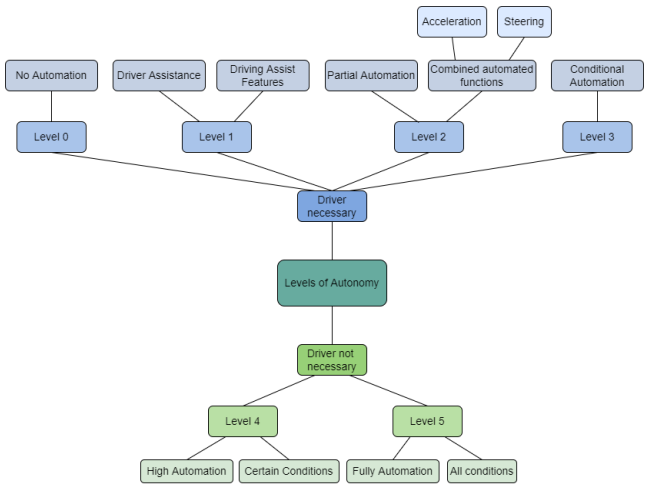
\includegraphics[width=\textwidth]{Figures/level-auto.png}
\caption{Níveis de Autonomia \cite{review-auto}.}
\label{niveis-auto}
\end{figure}

\begin{quote}
Descrição da figura \ref{niveis-auto}:  \textit{Nível 0} - Sem automação.  \textit{Nível 1} - Assistência ao motorista e funcionalidades de assistência.  \textit{Nível 2} - Automação parcial e funcionalidades de assistência combinadas.  \textit{Nível 3} - Automação condicionada.  \textit{Nível 4} - Alta automação em certas condições.  \textit{Nível 5} - Totalmente autônomo em todas as condições. 
\end{quote}



\subsection{Condução Autônoma e mercado tecnológico}

A inserção da Condução Autônoma no mercado dependerá da demanda de viagens por veículos, da infraestrutura de transporte, do grau de automação desses veículos, da taxa na qual os veículos autônomos são introduzidos no mercado, e da confiança da sociedade com essa categoria de transporte. 

Como visto, no gráfico (Gráfico \ref{Graph_EN}) os níveis de automação de 0 a 3 exigirão a presença de um motorista no veículo. O nível 4 a 5, não fazem a exigência de ter a presença de um motorista humano na tarefa de monitorar constantemente o ambiente de direção. 
Abrindo categorias inteiramente novas de viagens, com a não necessidade de um motorista humano para a realização do transporte da população \cite{notif}.

Nessa realidade, onde não há mais a necessidade de um condutor humano para o veículo (Carro de Passeio). Haverá a possibilidade das pessoas se engajarem em outras atividades, pois agora a sua atenção não precisa está direcionada em conduzir ou assistir o veículo para alcançar o destino programado. 


Entretanto, essa realidade, ainda, é algo para 2029 \cite{elpais} data em que El Pais dá como previsão para essa categoria de veículos estarem amplamente em operação. Por outro lado, atualmente, a direção autônoma ainda funciona como um assistente para o condutor; os assistindo em trocas de faixas, estacionamento, controle de velocidade, entre outras coisas. 

Nesse sentido, trabalham as marcas de luxo onde essas tecnologias são mais comuns, devido ao alto custo de desenvolvimento. Desse modo, os consumidores podem, já hoje, ter acesso a veículos autónomos. Entretanto, esses veículos são definidos como semi autônomos classificados como nível 2 (Gráfico \ref{Graph_EN}) SAE. As principais marcas estadunidenses automotivas que trabalham, hoje, como essa tecnologia são:  Tesla, Cadillac, Audi, BMW, Mercedes-Benz, Jaguar, Land Rover \cite{caio}. 
Dessas marcas a que representa maiores avanços, segundo as pesquisas, é a Mercedes-Benz, sendo  a primeira das marcas a começar a sua produção já em 2024 de veículos comerciais com nível 3 SAE \cite{mercedes3}.
No outro espectro, há os veículos de carona que têm como essência ser carros autônomos que operam no nível 4 e 5 SAE, comumente conhecidos como Táxi Robô. Na atualidade, apenas algumas empresas trabalham com essa categoria de veículo. Esses carros, hoje, se situam no nível 3 - 4 de autonomia, operando apenas em rotas já cadastradas em seus bancos de dados, portanto em locais já conhecidos e sem muitas chances de situações extremas, fora das suas bases de dados. 

As principais empresas que trabalham no desenvolvimento dessa categoria de veículo são, por exemplo:

\begin{enumerate}

   \item \textbf{Waymo (Alphabet):}
         Trabalhando com veículos no nível 4 SAE. Entretanto, fazendo uso de seres humanos de maneira remota para dar assistência aos seus veículos quando necessário \cite{waymo}. Atualmente, a Waymo, subsidiária da Alphabet, possui as mais altas competências, incluindo a mais extensa experiência em testes do mercado\cite{CAM};
   \item \textbf{Zoox (Amazon):}
         Sua frota de veículos de carona operam no nível 3 \cite{zoox};
   \item \textbf{Uber:}
         Atualmente, seus veículos trabalham em nível 3 e estão a realizar testes em nível 4 SAE. Cujo é o objetivo da empresa pois a indústria automotiva define esse nível como "atenção desligada” \cite{uber};
   \item \textbf{Mobileye (Intel):}
         A frota de veículos hoje opera em nível equivalente ao 4 SAE. A empresa busca a sua própria taxonomia de seus veículos \cite{mobileye}, \cite{mobileye1}.
\end{enumerate}

Lista completa das empresas no domínio dos sistemas de condução autónoma:


\begin{figure}[H]
\centering
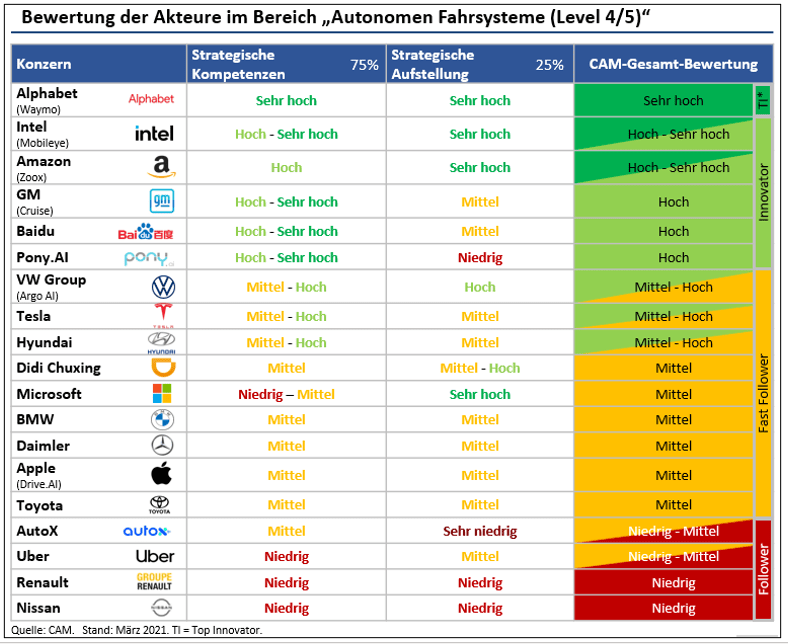
\includegraphics[width=16cm]{Figures/grafik.png}
\caption{Listas das empresas no domínio dos sistemas de condução autónoma (Nível 4/5) 2021 \cite{CAM}.}
\label{figura_companies}
\end{figure}

A partir dessa listagem \ref{figura_companies}, podemos ter uma melhor compreensão de como se encontra o cenário das empresas, na figura \textit{Konzern} em alemão, que hoje trabalham com veículos que possuem algum tipo de recurso autônomo, referente ao SAE \ref{SAE-level}. Listagem oriunda da (CAM) \textit{The Center of Automotive Management}; fornece com base em métodos científicos e bancos de dados abrangentes, orientações confiáveis sobre o universo automobilístico \cite{CAM}.

\subsubsection{VAs no mercado}

Decorrente  do aumento da automação industrial, há uma previsão do mercado mundial de veículos autônomos atingir US \$ 10 bilhões até 2024 \cite{mercadoo}. Essa previsão tem em vista o avanço da movimentação e armazenamento interno de materiais no ambiente industrial, a aplicação dos VAs nesse setor é uma tendência de mercado no interesse do investimentor \ref{implementacao}, pois os resultados gerados com a aplicação desse sistema impactam positivamente a empresa, a sociedade e a economia.

Ainda na perspectiva de crescimento econômico, e investimento no setor automobilístico em relação aos VAs. O CEO da GM, Mary Barra, diz estar investindo agressivamente no mercado de VA, com um plano de investimento de US \$35 bilhões para veículos movidos a bateria e autônomos. Tendo como expectativa arrecadar \$50 bilhões até o final da década \cite{gm}.

Além disso, espera-se que as implicações dos VAs influenciem diferentes aspectos do sistema econômico, além do industrial, e as empresas que não conseguirem se adaptar a essa mudança terão perdas significativas de mercado. Em geral, espera-se que o valor econômico dos VAs seja bem significativo e aumente com o tempo, abrindo novas oportunidades de negócios e profissões.

\begin{figure}[H]
\centering
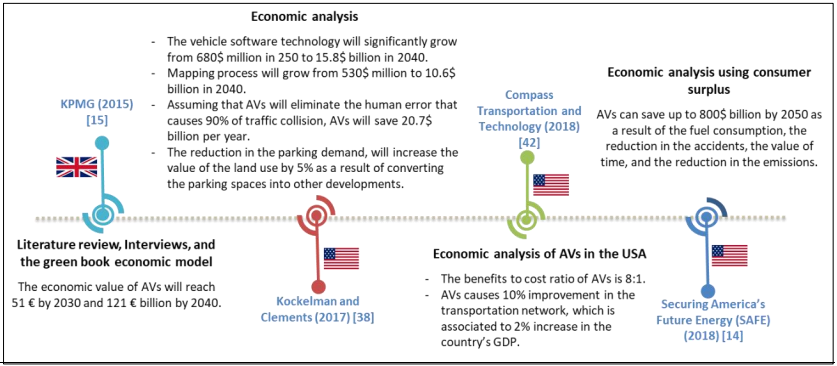
\includegraphics[width=\textwidth]{Figures/vas-mercado.png}
\caption{Resumo dos resultados de estudos anteriores que analisam o impacto dos VAs nas economias \cite{mundobrasil}.}
\label{figura_resumo}
\end{figure}

\begin{quote}
Descrição da figura \ref{figura_companies}: apresenta um panorama econômico e do que espera-se dos veículos autonomia para as próximas décadas. Prever que os VAs terão um valor econômico de 51 bilhões de euros em 2030 e até 2040 um valor de 121 bilhões de euros. A análise, também, apresenta que devido a redução da demanda de espaço para estacionamentos o valor dessas terras irão aumentar em 5\%, pois poderão ser utilizadas em outros propósitos. Ademais, os VAs podem salvar até 800 bilhões de dólares até 2050, devido a redução do consumo de combustível e acidentes de trânsito. 
\end{quote}

Em linhas gerais, o valor econômico dos VAs vem de sua capacidade de reduzir o erro humano e melhorar a segurança no trânsito em 90\%, usos como espaço de estacionamento poderão ser utilizados para outras atividades. Pois, agora, esses veículos podem ficar circulando pela cidade ou até mesmo voltar para a residência do proprietário e voltar para buscá-lo no horário estipulado \cite{4cenarios_ocidental}. De todo modo, haverá muitas novas oportunidades de negócios criadas oriundas dos VAs \cite{mundobrasil}.




\section{Tecnologias Essenciais para a Direção Autônoma}

\subsection{Como um veículo é automatizado}
Nesta seção cobrimos como um veículo é automatizado, seus componentes principais para se tornar um VA. Dentre as características que encontramos durante nossas pesquisas foram a percepção, planejamento e controle.

Como representado na figura a seguir (Figurac\ref{figura_perception}) um veículo necessita de 3 componentes essenciais para alcançar algum nível de automação SAE \ref{SAE-level}, sendo esses:


\begin{enumerate}
 \item \textbf{Percepção (Perception):} Busca entender o ambiente, fazendo uso de visão a partir de sensores \ref{sensores-a}, dados, localização, e redes de conexão à internet.
\item \textbf{Planejamento (Planning):} Planejamento de ação e trajetória, guia o veículo do início ao fim, missão de planejamento, planejamento de comportamento e movimento, e planejamento de tempo e da dinâmica do ambiente.
\item \textbf{Controle (Control):} Busca executar o planejamento deferido pela camada anterior, predizendo os controles para execução da tarefa designada, controle dos freios, acelerador e volante, geração da trajetória e controle da execução.

\end{enumerate}

\begin{figure}[H]
\centering
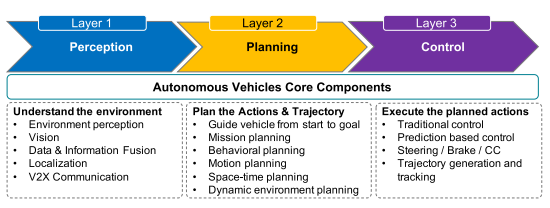
\includegraphics[width=\textwidth]{Figures/perception.png}
\caption{Componentes em camadas para obter um VA \cite{sensors-yet}.}
\label{figura_perception}
\end{figure}

As camadas representadas na figura acima (Figura \ref{figura_perception}) cada uma delas implementam diferentes operações e interagem entre si para realizar os casos de uso na direção autônoma. A figura abaixo (Figura\ref{figura_camadas}) representa essa comunicação entre camada e como essa interação acontece.

\begin{figure}[H]
\centering
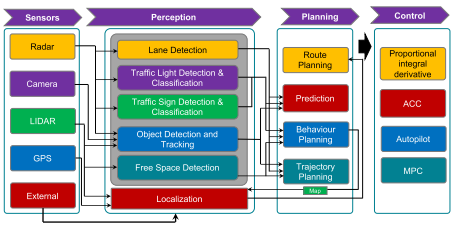
\includegraphics[width=\textwidth]{Figures/layer-sens.png}
\caption{Operações específicas de camadas e interações entre camadas. \cite{sensors-yet}.}
\label{figura_camadas}
\end{figure}



\subsection{Sensores e suas funções em Veículos Autônomos} \label{sensores-a}

Como apresentado nas seções anteriores, um VA é uma categoria de veículo que pode fazer sentido do que está ao seu redor e operar sem a necessidade de intervenção humana. Desse modo, para fazer sentido do que está em sua volta é necessário recursos para essa compreensão. Dentre esses recursos estão os sensores que são dispositivos que convertem eventos detectados ou mudanças no ambiente em uma medida numérica que pode então ser processada pelo componente de processamento central do veículo. 
Os sensores são divididos em duas categorias com base em seu princípio operacional \cite{sensors}: 

\begin{enumerate}
 \item \textbf{Sensores de estado interno:} Conhecidos como sensores proprioceptivos, registram o estado dinâmico de um sistema dinâmico e detectam dados internos como força, taxa angular, pressão da roda, voltagem da bateria e assim por diante. Unidades de medição inercial, codificadores, sensores inerciais (giroscópios e magnetômetros) e sensores de localização são exemplos de sensores proprioceptivos. 
\item \textbf{Sensores exteroceptivos:} São sensores de estado externo, por outro lado, percebem e coletam informações do ambiente do sistema, como medições de distância ou intensidade de luz. Os sensores externos incluem câmeras, detecção e alcance de rádio (Radar), detecção e alcance de luz (LiDAR) e sensores ultrassônicos.

\end{enumerate}



\begin{figure}[H]
\centering
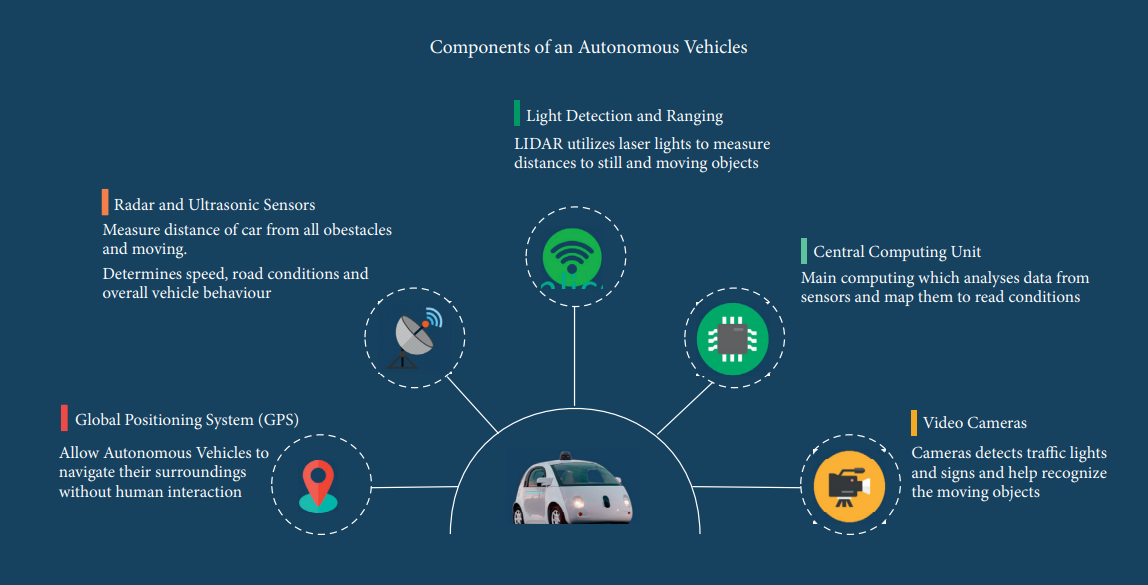
\includegraphics[width=\textwidth]{Figures/compo.png}
\caption{Componentes de um veículo autônomo \cite{aplicacao2}.}
\label{figura_compone}
\end{figure}

\begin{quote}
Descrição da figura \ref{figura_compone}. Componentes de um VA: \textit{GPS}; permite a navegação pelo ambiente sem interação do humano. \textit{RADAR e Sensores Ultra Sônicos}; calcula a distância de obstáculos, determinada a velocidade, condição da pista e as atividades do VA no geral. \textit{LiDAR}; utiliza luz para medir a distância de objetos parados e em movimento. \textit{Computador Central}; analise os dados dos sensores e os mapeiam para entender as condições do ambiente. \textit{Câmara de Vídeo}; detecção de semáforos, sinais de trânsito e objetos em movimento.
\end{quote}

 

\subsubsection{Visão geral sobre os sensores}

Esta seção é uma visão geral sobre diferentes tipos de sensores dos VAs com base em suas diferentes propriedades e aplicações. Examinamos, também, as vantagens e desvantagens dos três sensores básicos para percepção do ambiente utilizados do VAs na atualidade \cite{sensors}, e esses sensores são organizados como mostra a imagem abaixo:


\begin{figure}[H]
\centering
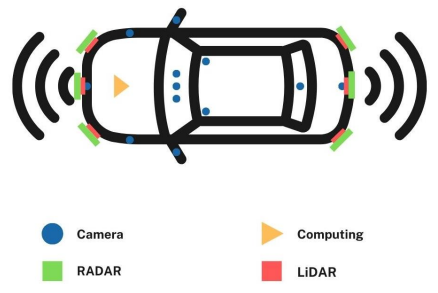
\includegraphics[width=8cm]{Figures/sensores.png}
\caption{Tipos de sensores em VAs. \cite{review-auto}.}
\label{figura-sensores}
\end{figure}


A conjugação desses sensores (Figura \ref{figura-sensores}) é o que possibilita os VAs. Desse modo, as figuras (Figuras \ref{tabela-juncao} e \ref{all-sense}) a seguir resumem essa comunicação didaticamente:

\begin{figure}[H]
\centering
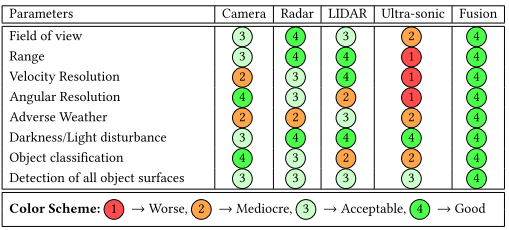
\includegraphics[width=10cm]{Figures/all-sense.png}
\caption{Adequação de sensores para diferentes situações. \cite{sensors-yet}.}
\label{all-sense}
\end{figure}
\begin{quote}
Descrição da tabela \ref{all-sense}: Apresenta parâmetros para comparação entre sensores, sendo os parâmetros: \textit{Campo de visão, distância, entendimento de velocidade, resolução de ângulo, clima adverso, escuridão/distorção de luz, classificação de objetos e detecção da superfície de objetos.} Esses parâmetros são classificados de Ruim (1), Pobre (2), Aceitável (3) e Bom (4).
\end{quote}

\begin{figure}[H]
\centering
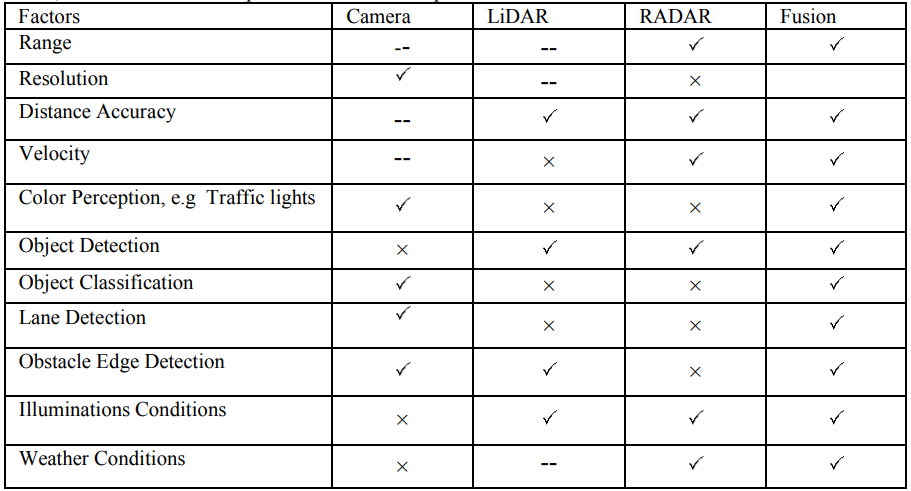
\includegraphics[width=12cm]{Figures/juncao-table.png}
\caption{Comparação comum entre sensores.}
\label{tabela-juncao}
\end{figure}
\begin{quote}
Descrição da tabela \ref{tabela-juncao}: "\checkmark" Os sensores operam completamente sob condições específicas,
"--" os sensores funcionam razoavelmente bem sob condições específicas, "x" os sensores não funcionam bem sob o fator específico em relação a outros sensores \cite{sensors}.
\end{quote}

\subsubsubsection{Câmeras}

As Câmeras são uma das tecnologias mais utilizadas para observar o ambiente. Uma câmera produz imagens nítidas dos arredores detectando as luzes emitidas de uma superfície fotossensível (plano de imagem) usando uma lente de câmera (colocada na frente do sensor) \cite{sensors}. Os VAs possuem esses sensores de luz visível para fornecer uma visão de 360 graus do ambiente. As câmeras são ótimos na detecção e reconhecimento de objetos, fornecendo detalhes mais ricos e ajudando a entender os objetos sem ou com profundidade, que geralmente não são detectados por outros tipos de sensores. Dentre esses objetos estão: Sinais de trânsito (limite de velocidade, sinais de parada, sinais de ultrapassagem), semáforos, pedestres, animais são alguns exemplos de tais objetos sem ou com profundidade \cite{sensors-yet}. Esses dados coletados com as câmeras são enviados para os algoritmos baseados em IA para uso posterior, e criação de uma imagem 2D \cite{aplicacao2}. 
No entanto, esses sensores são imprecisos em ambientes escuros e geram uma grande quantidade de dados para processar. Outros tipos de câmeras como as infravermelhas, também, são utilizadas para melhor desempenho em condições de baixa visibilidade \cite{review-auto}. As câmeras são dispostas nos VAs como mostrado na figura: (Figura \ref{figura-sensores}), e para detalhes específicos dos diferentes modelos de câmeras e suas características na tabela: (Tabela \ref{tabela-camera}).

\begin{figure}[H]
\centering
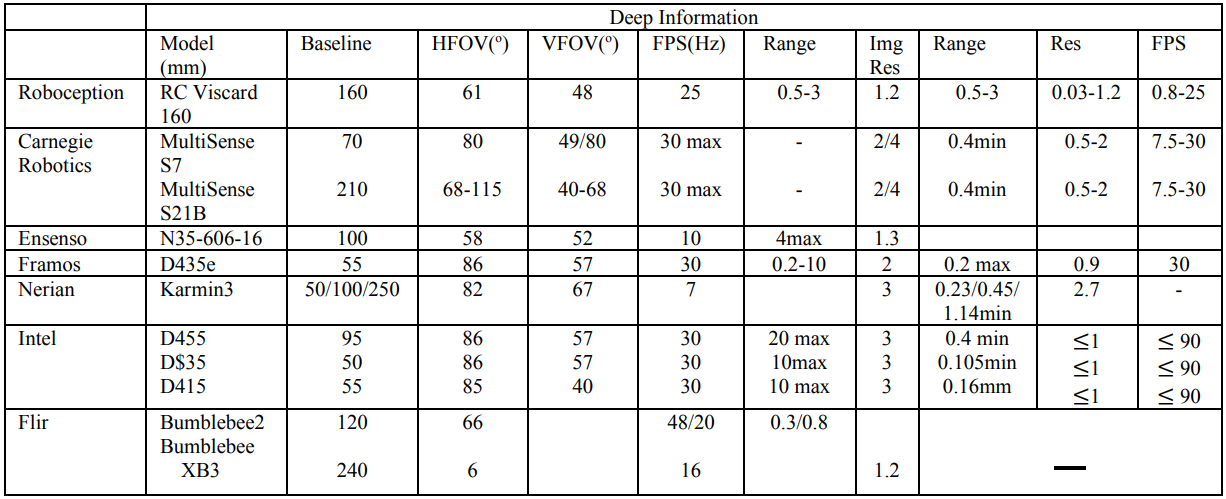
\includegraphics[width=\textwidth]{Figures/camera-table.png}
\caption{Especificações gerais da câmera estéreo.}
\label{tabela-camera}
\end{figure}
\begin{quote}
Descrição da tabela \ref{tabela-camera}: Campo de visão horizontal (HFOV), Campo de visão vertical (VFOV), Quadros por segundo (FPS), Resolução da imagem em megapixels (Res Img), Quadros de profundidade por segundo (FPS) \cite{sensors}.
\end{quote}
\subsubsubsection{LiDAR}

O LiDAR, ou detecção e alcance de luz, foi desenvolvido pela primeira vez na década de 1960 e desde então tem sido amplamente empregado no mapeamento de terreno aeronáutico e aeroespacial \cite{sensors}. Nos VAs os LiDAR são sensores que usa a luz como meio para medir distâncias é calculado medindo o tempo que a luz leva para ser refletida no receptor, e são dispostos no VA como mostrado na figura (Figura \ref{figura-sensores}) . Tais sistemas emitem feixes de laser que atingem o ambiente e refletem para um fotodetector. Os feixes coletados em tempo real e de maneira confiável, e  são convergidos juntos como uma nuvem de pontos criando uma imagem 3D do ambiente \cite{aplicacao2}. Dado que os LIDARs são sensores sem profundidade, eles não são capazes de identificar os elementos sem profundidade, como semáforos, sinais de trânsito e assim por diante.
Embora o LiDAR seja um sensor poderoso e eficiente para o uso em VAs, acabam por ser  bastante caros e aumentando o valor final do VA \cite{review-auto}. 
Os LiDAR em VAs são dispostas como mostrado na figura (Figura \ref{figura-sensores}), e para mais detalhes específicos e diferentes características do LiDAR, verificar a seguinte tabela: (Tabela \ref{tabela-lidar}).

\begin{figure}[H]
\centering
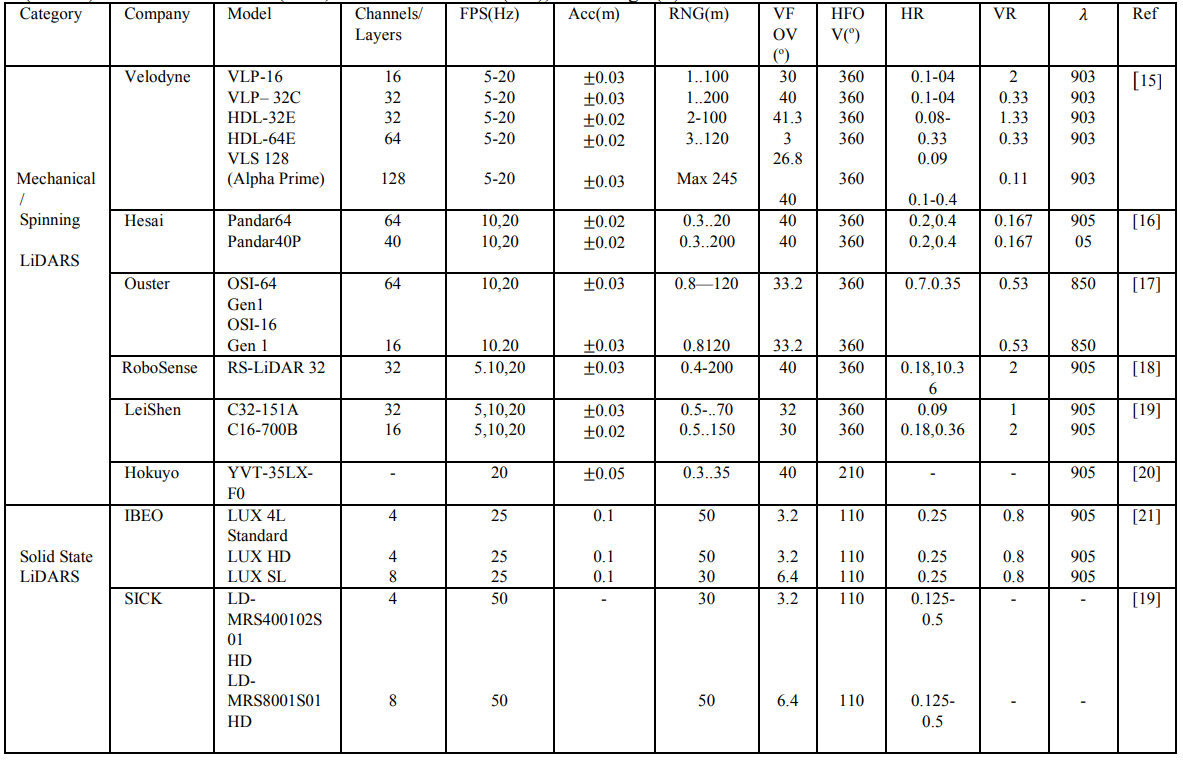
\includegraphics[width=\textwidth]{Figures/lidar-table.png}
\caption{Especificações gerais de LiDAR.}
\label{tabela-lidar}
\end{figure}

\begin{quote}
Descrição da tabela \ref{tabela-lidar}: Quadro por segundo (FPS), Precisão (Acc), Alcance de detecção (RNG), FoV vertical (VFOV), FoV horizontal (HFOV) Resolução horizontal (HR0, Resolução vertical (VR), Comprimento de onda ($\lambda$) \cite{sensors}.
\end{quote}


\subsubsubsection{Radares}



Antes da Segunda Guerra Mundial, foi desenvolvido o \textit{Radio Detection and Ranging}, ou Radar. Tem como essência emitir ondas eletromagnéticas dentro da região de interesse e receber ondas dispersas (ou reflexões) de alvos para processamento de sinal e determinação a informações que alcançam \cite{sensors}. Trabalhando com essas ondas de rádio para calcular fatores como a distância, velocidade e ângulo. Com a ajuda desses transmissores de radar, os VAs podem emitir ondas de rádio e receber as ondas refletidas com a ajuda de receptores de radar. O radar funciona bem na maioria dos climas e em longas distâncias, mas pode identificar objetos falsamente \cite{review-auto}.
Os Radares em VAs são dispostas como mostrado na (Figura \ref{figura-sensores}), e para mais detalhes específicos e diferentes características dos Radares, verificar a seguinte tabela: (Tabela \ref{tabela-radar}).



\begin{figure}[H]
\centering
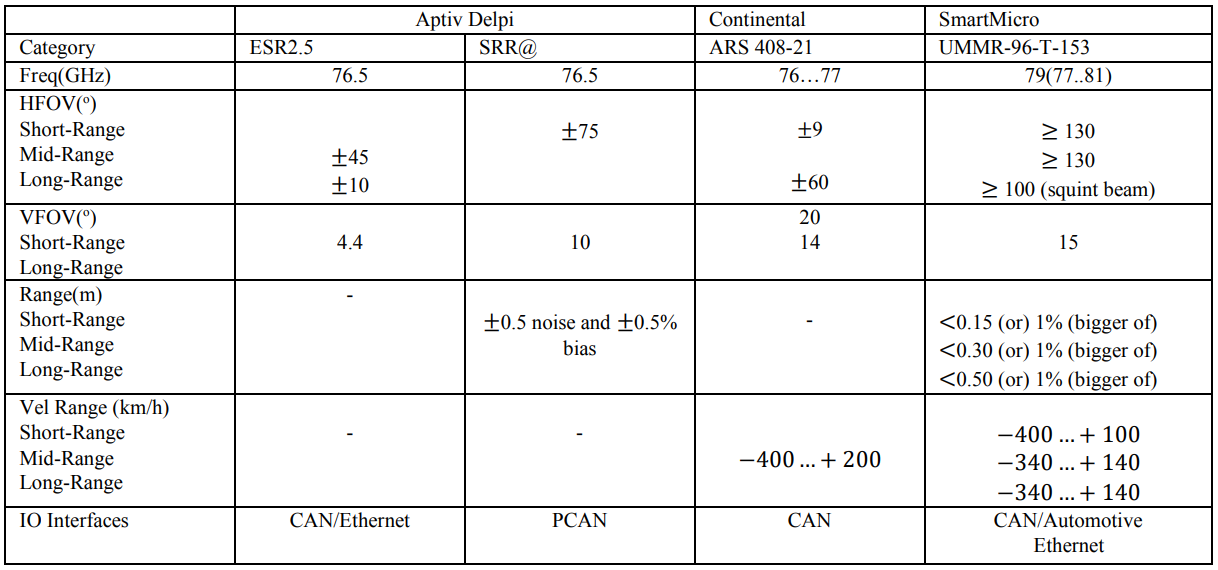
\includegraphics[width=\textwidth]{Figures/radar-table.png}
\caption{Especificação geral de sensores RADAR.}
\label{tabela-radar}
\end{figure}

\begin{quote}

Descrição da tabela \ref{tabela-radar}:  Acrônimos primeiro da primeira coluna de cima para baixo, Frequência (Freq), FoV horizontal (HFOV), FoV vertical (VFOV), Precisão de alcance (Faixa Acc), Faixa de velocidade (Faixa Vel), ROS (Sistema operacional robótico) \cite{sensors}.
\end{quote}


\subsubsection{Sistemas avançados de assistência ao condutor}


Como apresentado em seções anteriores, os VAs possuem tecnologias de assistência ao condutor ou ADAS visando aumentar a segurança e conforto dos VAs. Essas tecnologias de assistência ao motorista são comumente empregadas nos VAs de nível 1 a 3 SAE \ref{SAE-level}.

\subsubsubsection{Controle de Cruzeiro}

O Controlador de Cruzeiro foi introduzido pela primeira vez no mercado automotivo na década de 1980, o controle de cruzeiro apareceu no início do século XX, operado por um dispositivo chamado regulador centrífugo que regulava a velocidade com base na quantidade de combustível injetado \cite{caio}. Essa funcionalidade é capaz de ajustar automaticamente a velocidade do veículo mantendo uma distância constante do veículo seguinte \cite{sensors-yet}.
A partir disso os VAs são capazes de evitar possíveis colisões, emitindo sinais sonoros para o condutor, e reduzindo a velocidade do veículo até alcançar uma distância segura. Na atualidade, esse sistema é conhecido como controle de cruzeiro adaptativo ou \textit{Adaptive Cruise Control} (ACC) baseado em radares que, ainda, mede a distância, velocidade e ângulo de aproximação entre os carros nas estradas como ilustrado nas imagens a seguir: \ref{cruzeiro} e \ref{ACC}:

\begin{figure}[H]
\centering
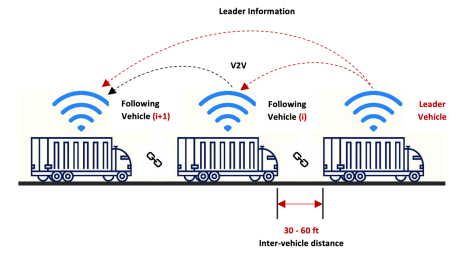
\includegraphics[width=10cm]{Figures/cruzeiro.png}
\caption{Distância entre veículos \cite{review-auto}.}
\label{cruzeiro}
\end{figure}


\begin{figure}[H]
\centering
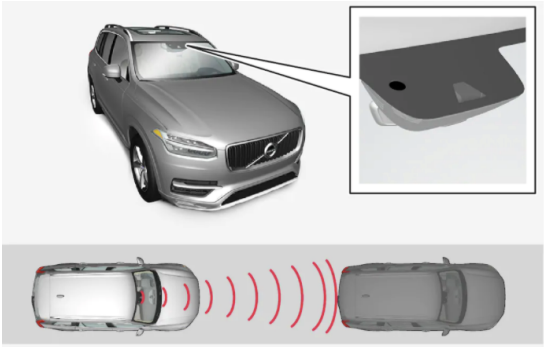
\includegraphics[width=10cm]{Figures/ACC.png}
\caption{Controle de Cruzeiro adaptativo em um carro da Volvo \cite{caio}.}
\label{ACC}
\end{figure}


\subsubsubsection{Assistente de permanência na faixa}

Assistente de Permanência na Faixa auxilia o motorista a manter o veículo na faixa e emite avisos quando o veículo sai da faixa. Também é muito útil para avisar os motoristas quando eles estão cansados \cite{caio}. A seguir a figura (Figura \ref{assistente}) apresenta o funcionamento do assistente:

\begin{figure}[H]
\centering
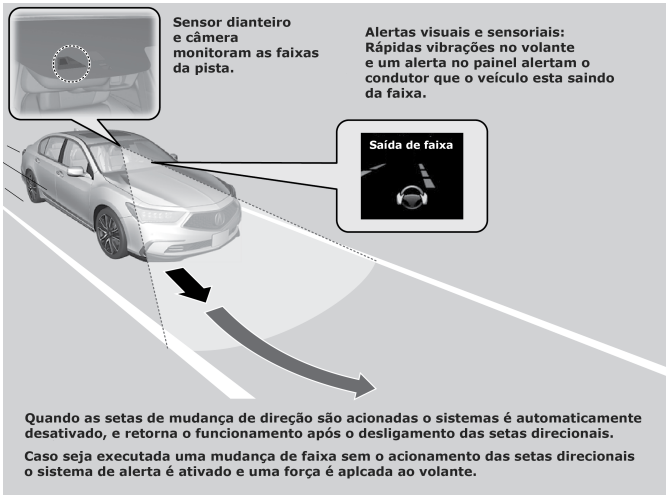
\includegraphics[width=\textwidth]{Figures/assistente.png}
\caption{Funcionamento do assistente de permanência de faixa \cite{caio}.}
\label{assistente}
\end{figure}

\subsubsubsection{Assistente de estacionamento}


A principal fonte dessa seção nos apresenta que um sistema de assistência ao estacionamento, também conhecido por Park Assist, tem como objetivo realizar as manobras de estacionamento de forma autónoma. Por meio de sensores (Figura \ref{figura-sensores}) ao redor do veículo, o sistema calcula o tamanho da folga (Figura \ref{cruzeiro}) e faz o movimento necessário para estacionar o veículo com total segurança. O carro assume o controle da direção e dos pedais, evitando qualquer obstáculo, mas o motorista deve estar sempre atento a qualquer imprevisto \cite{caio}.

\subsection{Arquiteturas e Algoritmos}

\subsubsection{Inteligência artificial}

Ao longo da história, os seres humanos tiveram que aprender e realizar tarefas que dependiam da inteligência para serem executadas, desde cálculos a programação de software até a condução de um veículo. Muito esforço tem sido feito nas últimas décadas para desenvolver vários sistemas de computação capazes de substituir humanos nessas tarefas, e muito dessa pesquisa para construir esse tipo de sistema pode ser atribuído ao campo da inteligência artificial \cite{caio}. 
Existem muitas definições para IA e seus sub campos, muitas das quais baseadas nas capacidades e comportamentos de um agente sob uma visão de domínio, o que significa que um agente pode ser definido operacionalmente em termos do ambiente em que atua.
Um agente deve ter as seguintes características principais, como: Autonomia, o que significa que ele pode tomar a iniciativa e exercer controle sobre suas ações, e conduzir negociações com agentes humanos ou outros para atualizar e melhorar as regras básicas.
Essas características são com base em estratégias de argumentação, o agente pode tomar decisões e tirar conclusões. Em geral, a inteligência artificial refere-se à capacidade de um computador ou máquina de imitar as habilidades da mente humana \cite{software-ia}. Existe uma relação entre os significados de inteligência artificial (IA), aprendizado de máquina (ML) e aprendizado profundo (DL), que é o seguinte: Os campos de inteligência artificial abrangem qualquer coisa relacionada a sistemas especialistas que tomam decisões com base em regras complexas.

\subsubsubsection{Aprendizado de Máquina}

O Aprendizado de Máquina está presente em muitas atividades da vida humana diária, por ex:. ao projetar a forma como uma rede social é apresentada a cada usuário, que tipo de anúncios e matérias são exibidos dependendo das preferências e consultas de pesquisa do usuário, separando e-mail confiável de spam e até câmeras de celular e teclado. Fazendo uso de algoritmos para coletar dados, permitindo que os computadores resolvam problemas e tomem decisões com base em seu próprio conhecimento adquirido ao longo do tempo \cite{caio}.



\chapter{Conclusões} \label{concl}


\chapter{Perspectiva de continuidade} \label{continuidade}
A partir da construção dos fundamentos da ciência de dados, identificamos diversas oportunidades de desenvolvimentos futuros, principalmente nas áreas de Data Visualization, Bancos de Dados e Aprendizado de Máquina. Especialmente na possibilidade de nos aprofundarmos em seus corpus de conhecimento e aplicá-los em projetos reais. 

\chapter{Participação em congressos e trabalhos publicados ou submetidos e outras
atividades acadêmicas e de pesquisa} \label{eventos}

Também apresentamos os certificados dos minicursos oferecidos pela plataforma Instituto de Tecnologia e Sociedade e Coursera  nas figuras \ref{Google} \ref{Design} e \ref{Direitos}.


\begin{figure}[H]
\centering
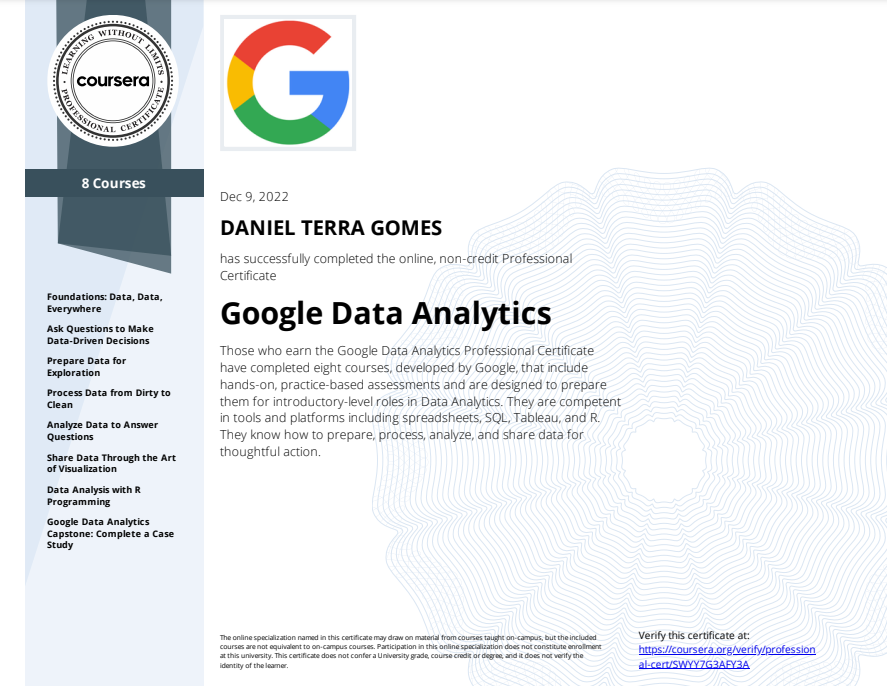
\includegraphics[width=\textwidth]{Figures/google.png}
\caption{Certificado de conclusão do curso Google Data Analytics.}
\label{Google}
\end{figure}

\begin{figure}[H]
\centering
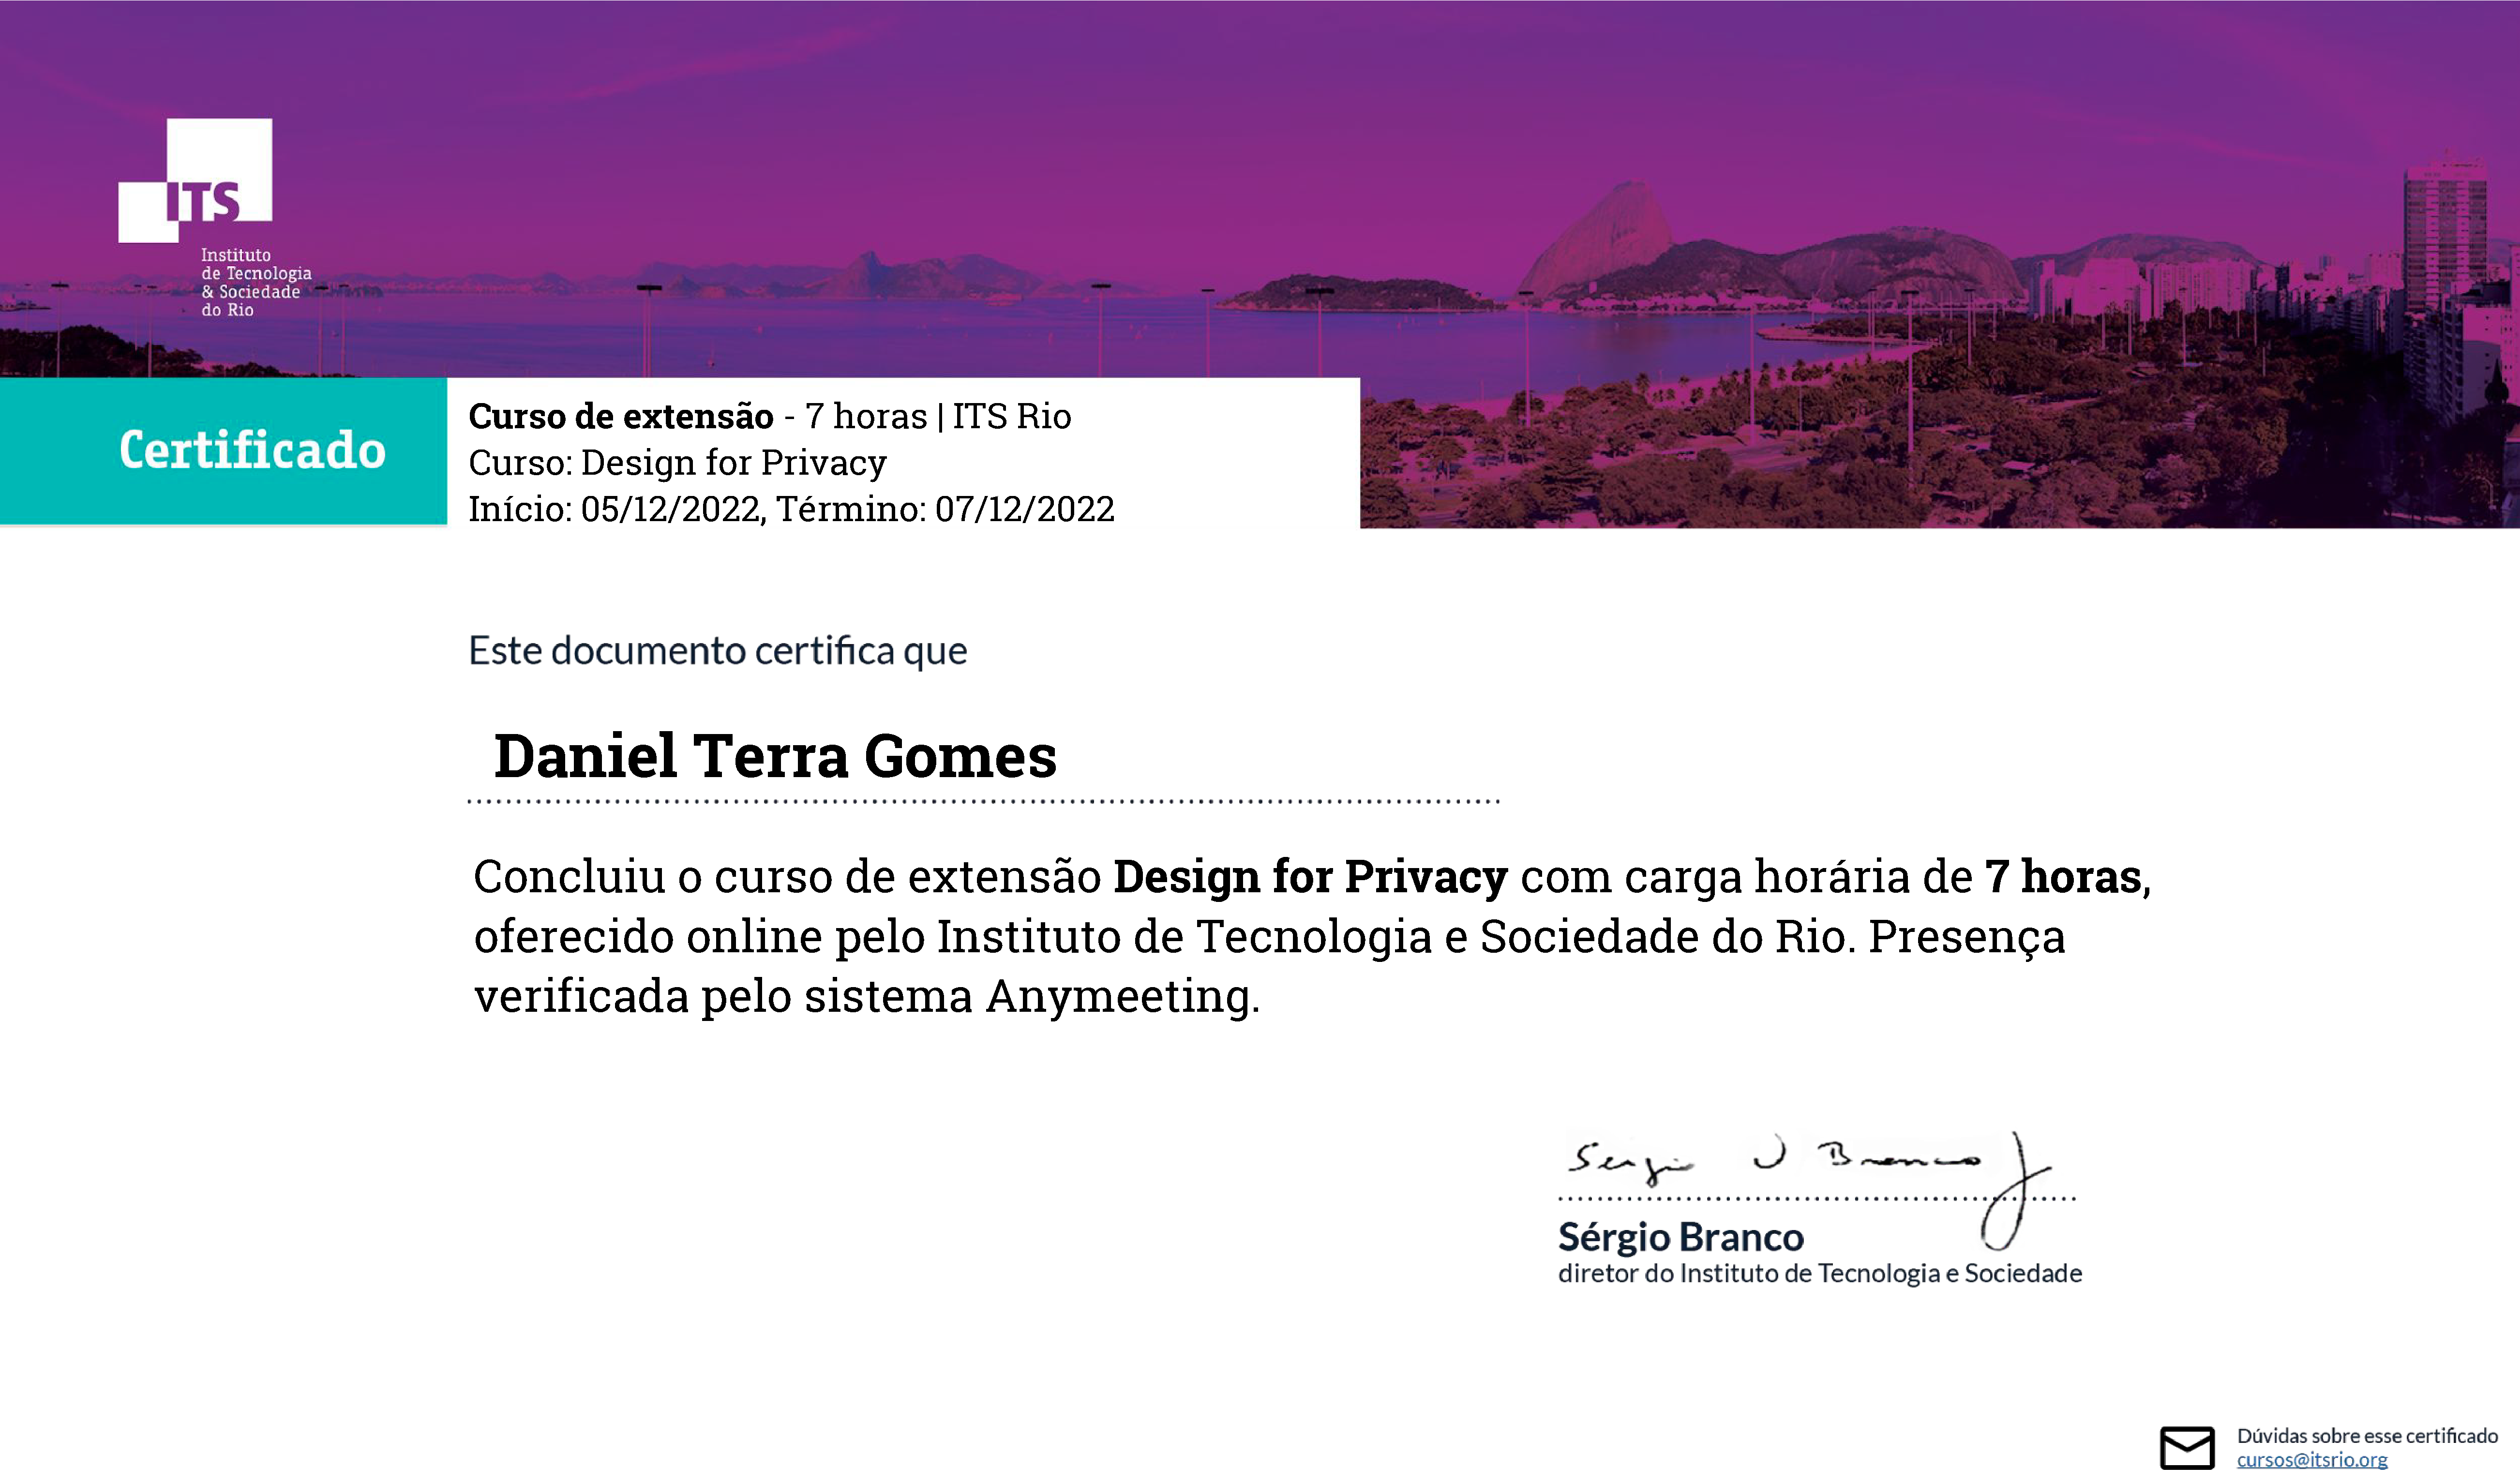
\includegraphics[width=\textwidth]{Figures/its2.pdf}
\caption{Certificado de conclusão ao curso Direitos humanos e Inteligência Artificial.}
\label{Direitos}
\end{figure}

\begin{figure}[H]
\centering
    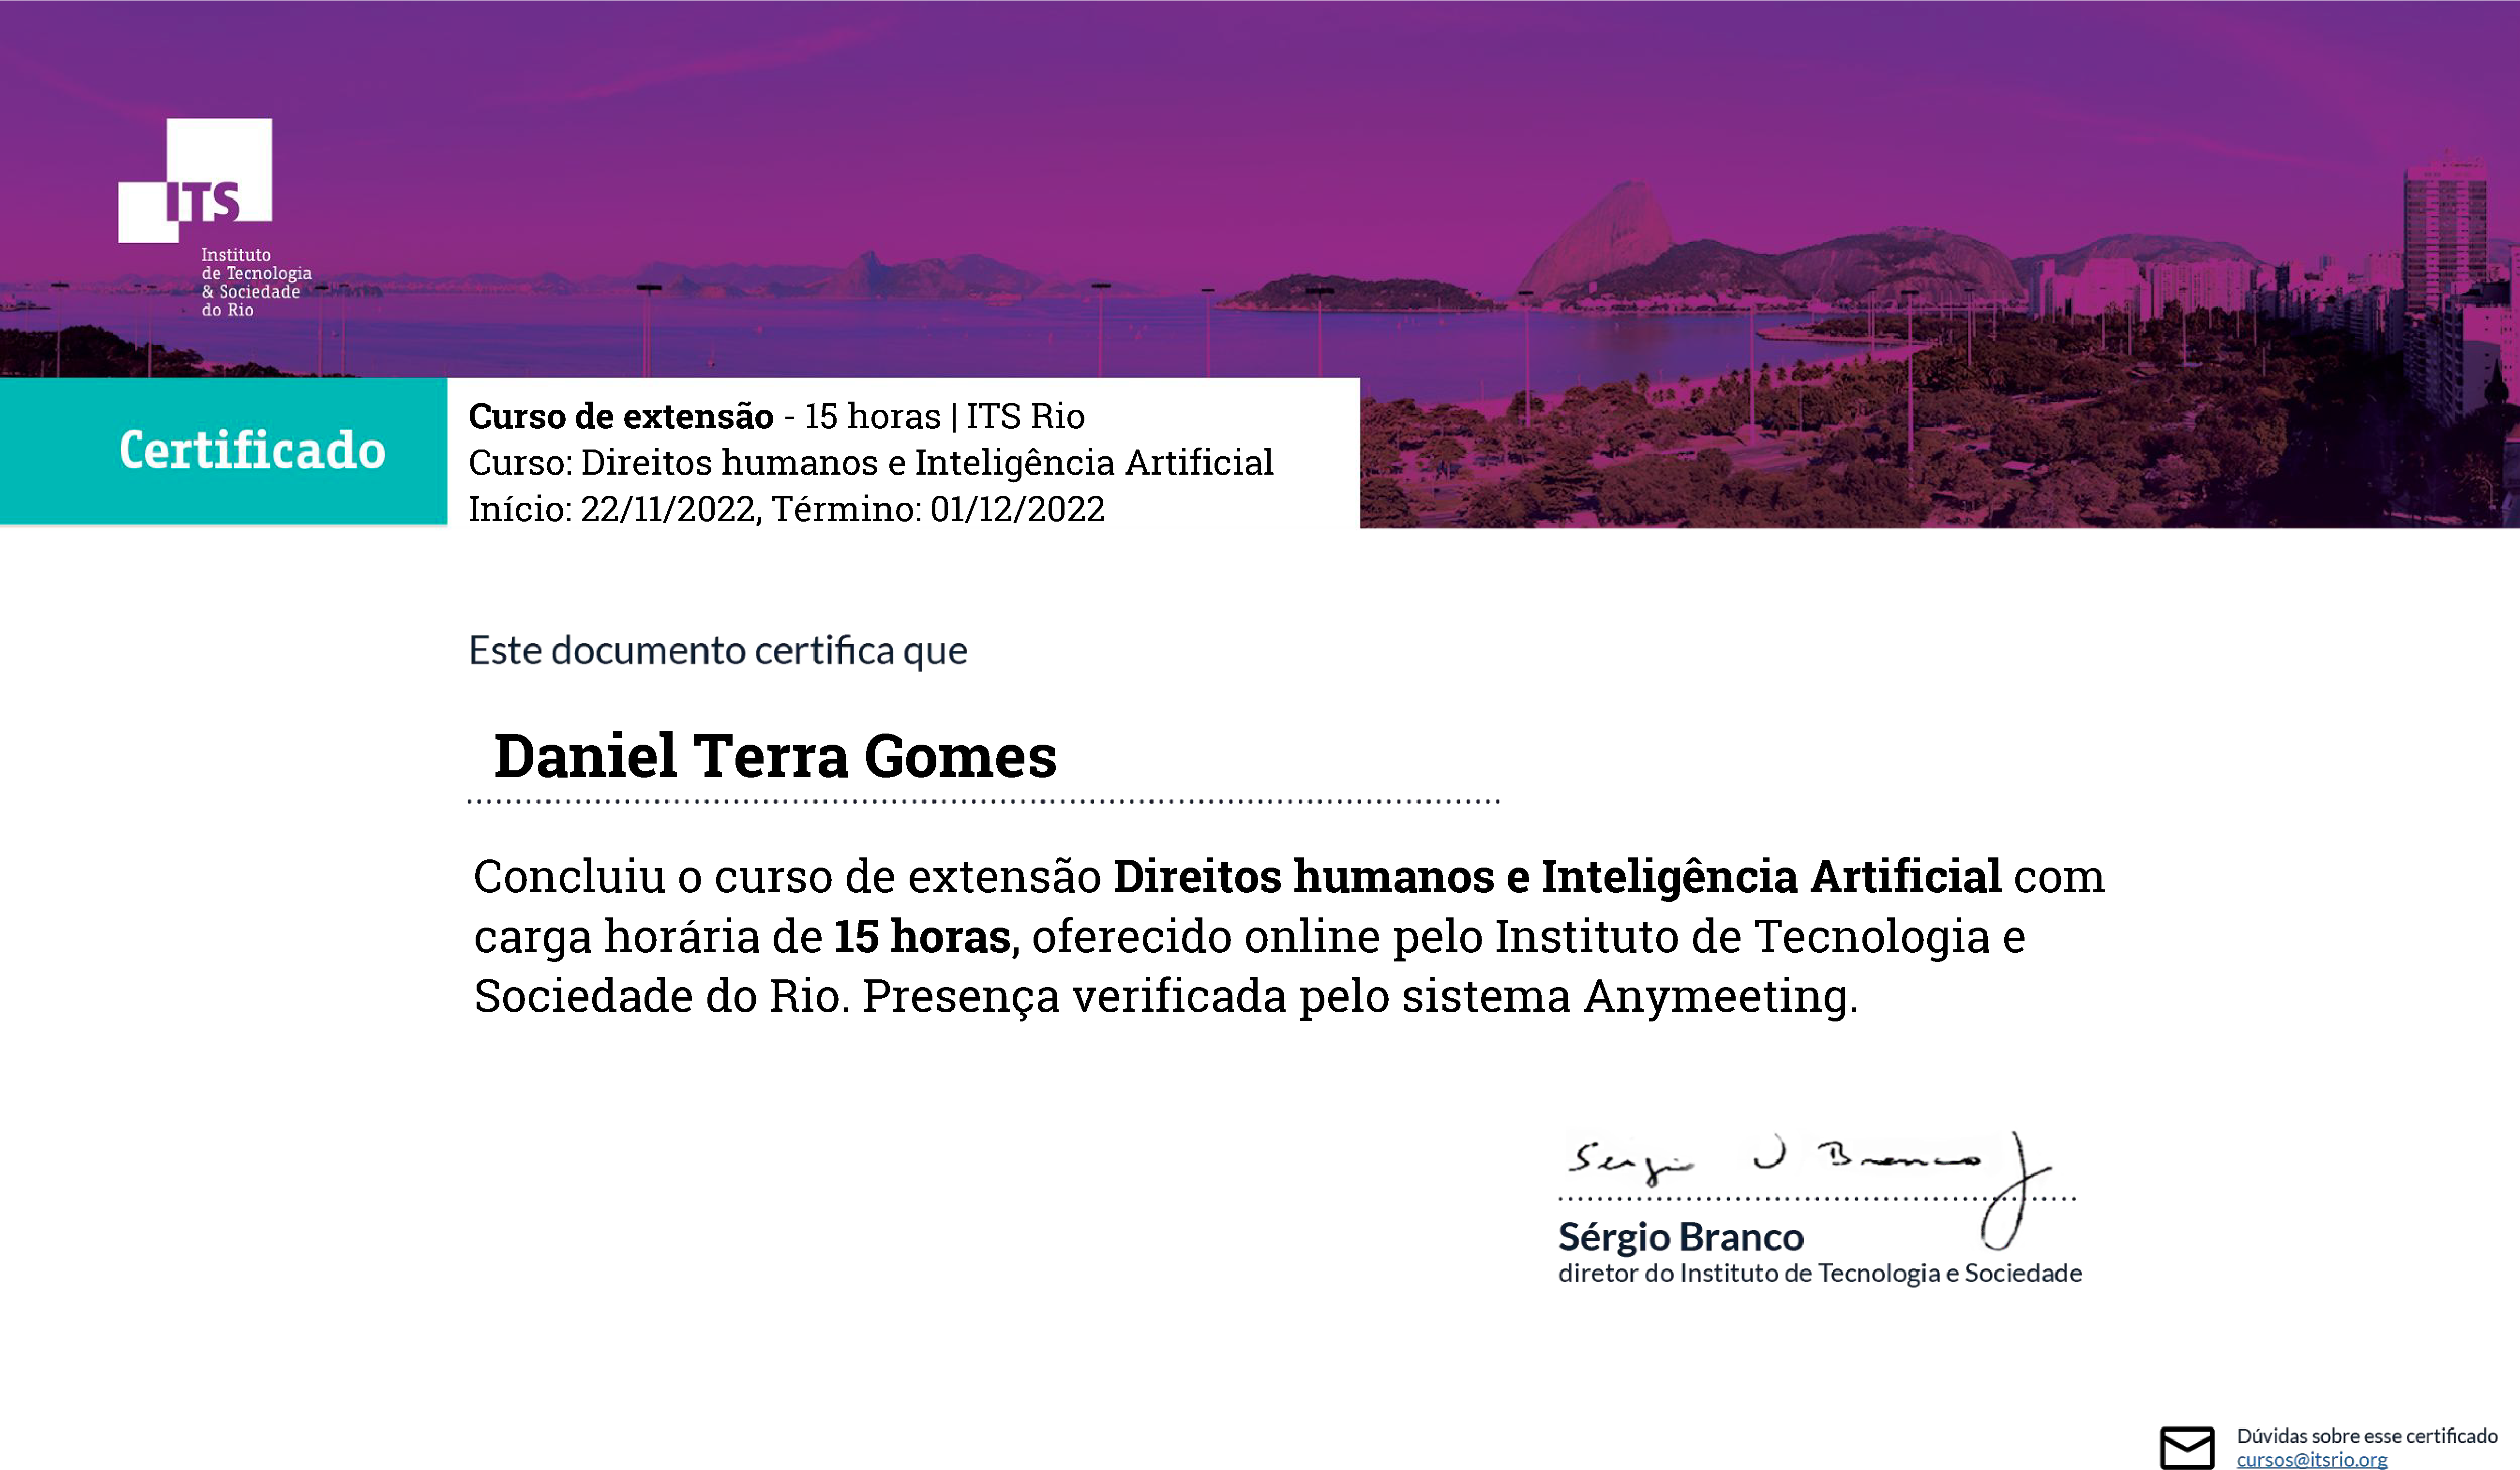
\includegraphics[width=\textwidth]{Figures/its1.pdf}
\caption{Certificado de conclusão ao curso Design for Privacy.}
\label{Design}
\end{figure}



\chapter{Datas e assinaturas} \label{ass}

\section{Data e assinatura do bolsista (assinatura digitalizada)}


\begin{figure}[H]
 \centering
 
\includegraphics[width=0.4\textwidth]{Figures/sign.png}
 %\caption{\label{kaggle.score}Pontuação final no Kaggle.}
\end{figure}
\center30/04/2023

\section{Data e assinatura do orientador (assinatura digitalizada)}


\begin{figure}[H]
 \centering
 
\includegraphics[width=0.4\textwidth]{Figures/assinatura_annabell.png}
 %\caption{\label{kaggle.score}Pontuação final no Kaggle.}
\end{figure}
\center 30/04/2023

